\documentclass[compress,aspectratio=169,10pt,usenames,dvipsnames]{beamer}

\mode<presentation>

\setbeamertemplate{theorems}[numbered]

\usetheme{CalPoly2023}

% use if you want greyed out steps rather than invisible
%\setbeamercovered{transparent}	

%Path relative to the main .tex file 
\graphicspath{ {./images} }

\usepackage{graphicx, amsmath, amsthm, amssymb, enumerate, esint, mathtools,multirow}
\usepackage{amsfonts,mathrsfs,float,array}
%\usepackage{xypic}
%\usepackage{tikz-cd}
\usepackage{tikz}
\usetikzlibrary{arrows, shapes, decorations}
%\usepackage{pgfplots}
%\usepackage{rotating}
%\usepackage[shortlabels]{enumitem}
\usepackage{subfigure}
\usepackage{multicol}
%\usepackage{amsmath}
%\usepackage{epsfig}
%\usepackage{graphicx}
%\usepackage[all,knot]{xy}
%\xyoption{arc}
\usepackage{url}
\usepackage{multimedia}
%\usepackage[usenames,dvipsnames]{xcolor}

\newcommand{\R}[1]{\mathbb{R}^{#1}}
\newcommand{\twobytwo}[4]{\left(\begin{array}{cc}
#1 & #2  \\
#3 & #4 \end{array} \right)}
\newcommand{\threebythree}[9]{\left( \begin{array}{ccc}
#1 & #2 & #3 \\
#4 & #5 & #6 \\
#7 & #8 & #9 \end{array} \right)}
\newcommand{\fourbyfour}[9]{\left( \begin{array}{cccc}
#1 & #2 & \cdots & #3 \\
#4 & #5 & \cdots & #6\\
\vdots & \vdots & \cdots  & \vdots \\
#7 & #8 & \cdots & #9 \end{array} \right)}
\newcommand{\ip}[2]{\left<  #1, #2 \right> }


%\theoremstyle{plain}
\newtheorem{prop}[theorem]{Proposition}
\newtheorem{conj}[theorem]{Conjecture}

%https://tex.stackexchange.com/questions/237949/theorem-and-proposition-with-arbitrary-number-in-beamer
%\newcommand{\propnumber}{} % initialize
%\newtheorem*{prop}{Proposition \propnumber}
%\newenvironment{propc}[1]
%  {\renewcommand{\propnumber}{#1}%
%   \begin{shaded}\begin{prop}}
%  {\end{prop}\end{shaded}}

\addtobeamertemplate{navigation symbols}{}{%
    \usebeamerfont{footline}%
    \usebeamercolor[fg]{footline}%
    \hspace{1em}%
    {\footnotesize \insertframenumber/\inserttotalframenumber}
}



\title[Math 442]{Math 442: Applications of Geometry \\ \;}
\author[Sean Gasiorek (gasiorek@calpoly.edu)]{Sean Gasiorek (gasiorek@calpoly.edu)}
\institute[Cal Poly]{}%{California Polytechnic State University} 
\date{March 13, 2024}
\setbeamercolor{section}{use=structure,fg=CPwhite,bg=CPgreen}
\setbeamercolor{section in head/foot}{use=structure,fg=CPwhite,bg=CPgreen}
\setbeamercolor{block title}{use=structure,fg=CPwhite,bg=CPgreen}
\setbeamercolor{block body}{use=structure,fg=black,bg=CPbeige}

\useoutertheme[subsection=false]{smoothbars}
%\setbeamertemplate{footline}[text line]{} % makes the footer EMPTY

%\usepackage{beamerouterthemesmoothbars}
% outer themes include default, infolines, miniframes, shadow, sidebar, smoothbars, smoothtree, split, tree

%%%%%%%%%%%%%%THIS WAS A ~26 MINUTE PRESENTATION WITH ALL VISIBLE SLIDES AND NO QUESTIONS DURING THE TALK


\listfiles
\begin{document}

\begin{frame}
\titlepage

\end{frame}

%%%%%%%%%%%%%%%%%%%%%%%%%%%%%%%%%%%%%%%%%%%%%%%%%%%%%%%%%%%%%%%%%%%%

%\begin{frame}
%\tableofcontents
%\end{frame}
\begin{frame}
\textbf{Outline:}
\begin{enumerate}
	\item Celestial Navigation
	\item Mathematical Billiards (my research area)
	\item More Geometry, More Billiards! (also my research area)
\end{enumerate}
\end{frame}


%%%%%%%%%%%%%%%%%%%%%%%%%%%%%%%%%%%%%%%%%%%%%%%%%%%%%%%%%%%%%%%%%%%%%


\section{Celestial Navigation}
\begin{frame}
  \sectionpage
\end{frame}

%%%%%%%%%%%%%%%%%%%%%%%%%%%%%%%%%%%%%%%%%%%%%%%%%%%%%%%%%%%%%%%%%%%%%

\begin{frame}

\vfill

\begin{block}{Question}
On a clear night, how can you tell which direction is north by looking at the stars? 
\end{block}
%\vskip10pt

\vfill

\onslide<2->
\begin{block}{Answer}
By finding the north star (also known as Polaris)! From where you're standing, the star will be roughly pointing in the northern direction. Or, geometrically speaking, minimize the distance from the north star to the horizon, and that point on the horizon will be north from wherever you happen to be. 
\end{block}

\vfill

\onslide<3->
\begin{block}{Follow-up Question}
But how do we find the north star?
\end{block}

\vfill

%\begin{center}
%%set up to be used in the 16:9 aspect ratio
%\begin{overlayarea}{11cm}{4cm}
%\begin{center}
%\includegraphics<1>[width=0.73\textwidth]{InitialSystem0}
%\includegraphics<2>[width=0.73\textwidth]{InitialSystem1}
%\includegraphics<3>[width=0.73\textwidth]{InitialSystem2}
%\includegraphics<4>[width=0.73\textwidth]{InitialSystem3}
%\includegraphics<5>[width=0.73\textwidth]{InitialSystem4}
%\end{center}
%\end{overlayarea}
%\end{center}


\end{frame}

%%%%%%%%%%%%%%%%%%%%%%%%%%%%%%%%%%%%%%%%%%%%%%%%%%%%%%%%%%%%%%%%%%%%%

\begin{frame}

\begin{center}
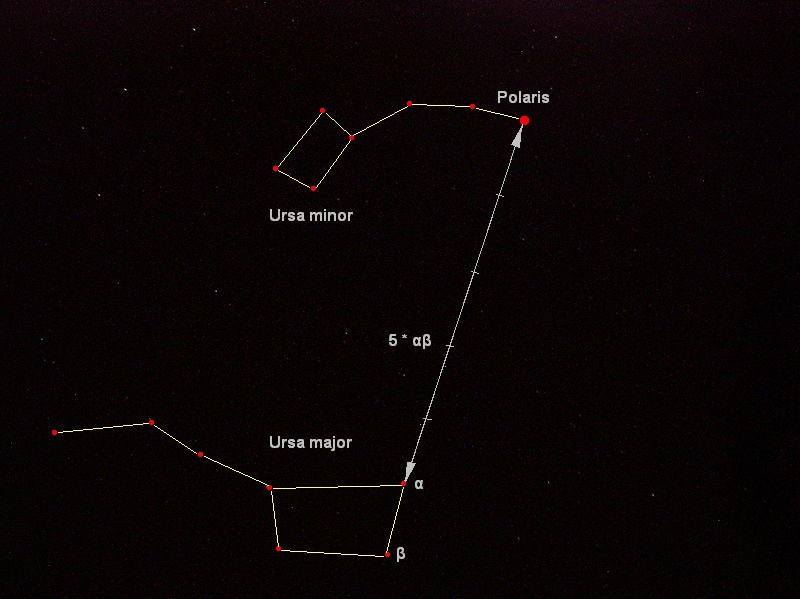
\includegraphics[width=0.73\textwidth]{Polaris} \\
{\tiny Source: {\tt https://en.wikipedia.org/wiki/Polaris}}
\end{center}

\end{frame}


%%%%%%%%%%%%%%%%%%%%%%%%%%%%%%%%%%%%%%%%%%%%%%%%%%%%%%%%%%%%%%%%%%%%%%

\begin{frame}

The north star also appears in a variety of contexts, from literature, history, religion, and exploration. It also plays an important role in Indigenous and First Nations culture.

\begin{center}
\begin{tabular}{c c}
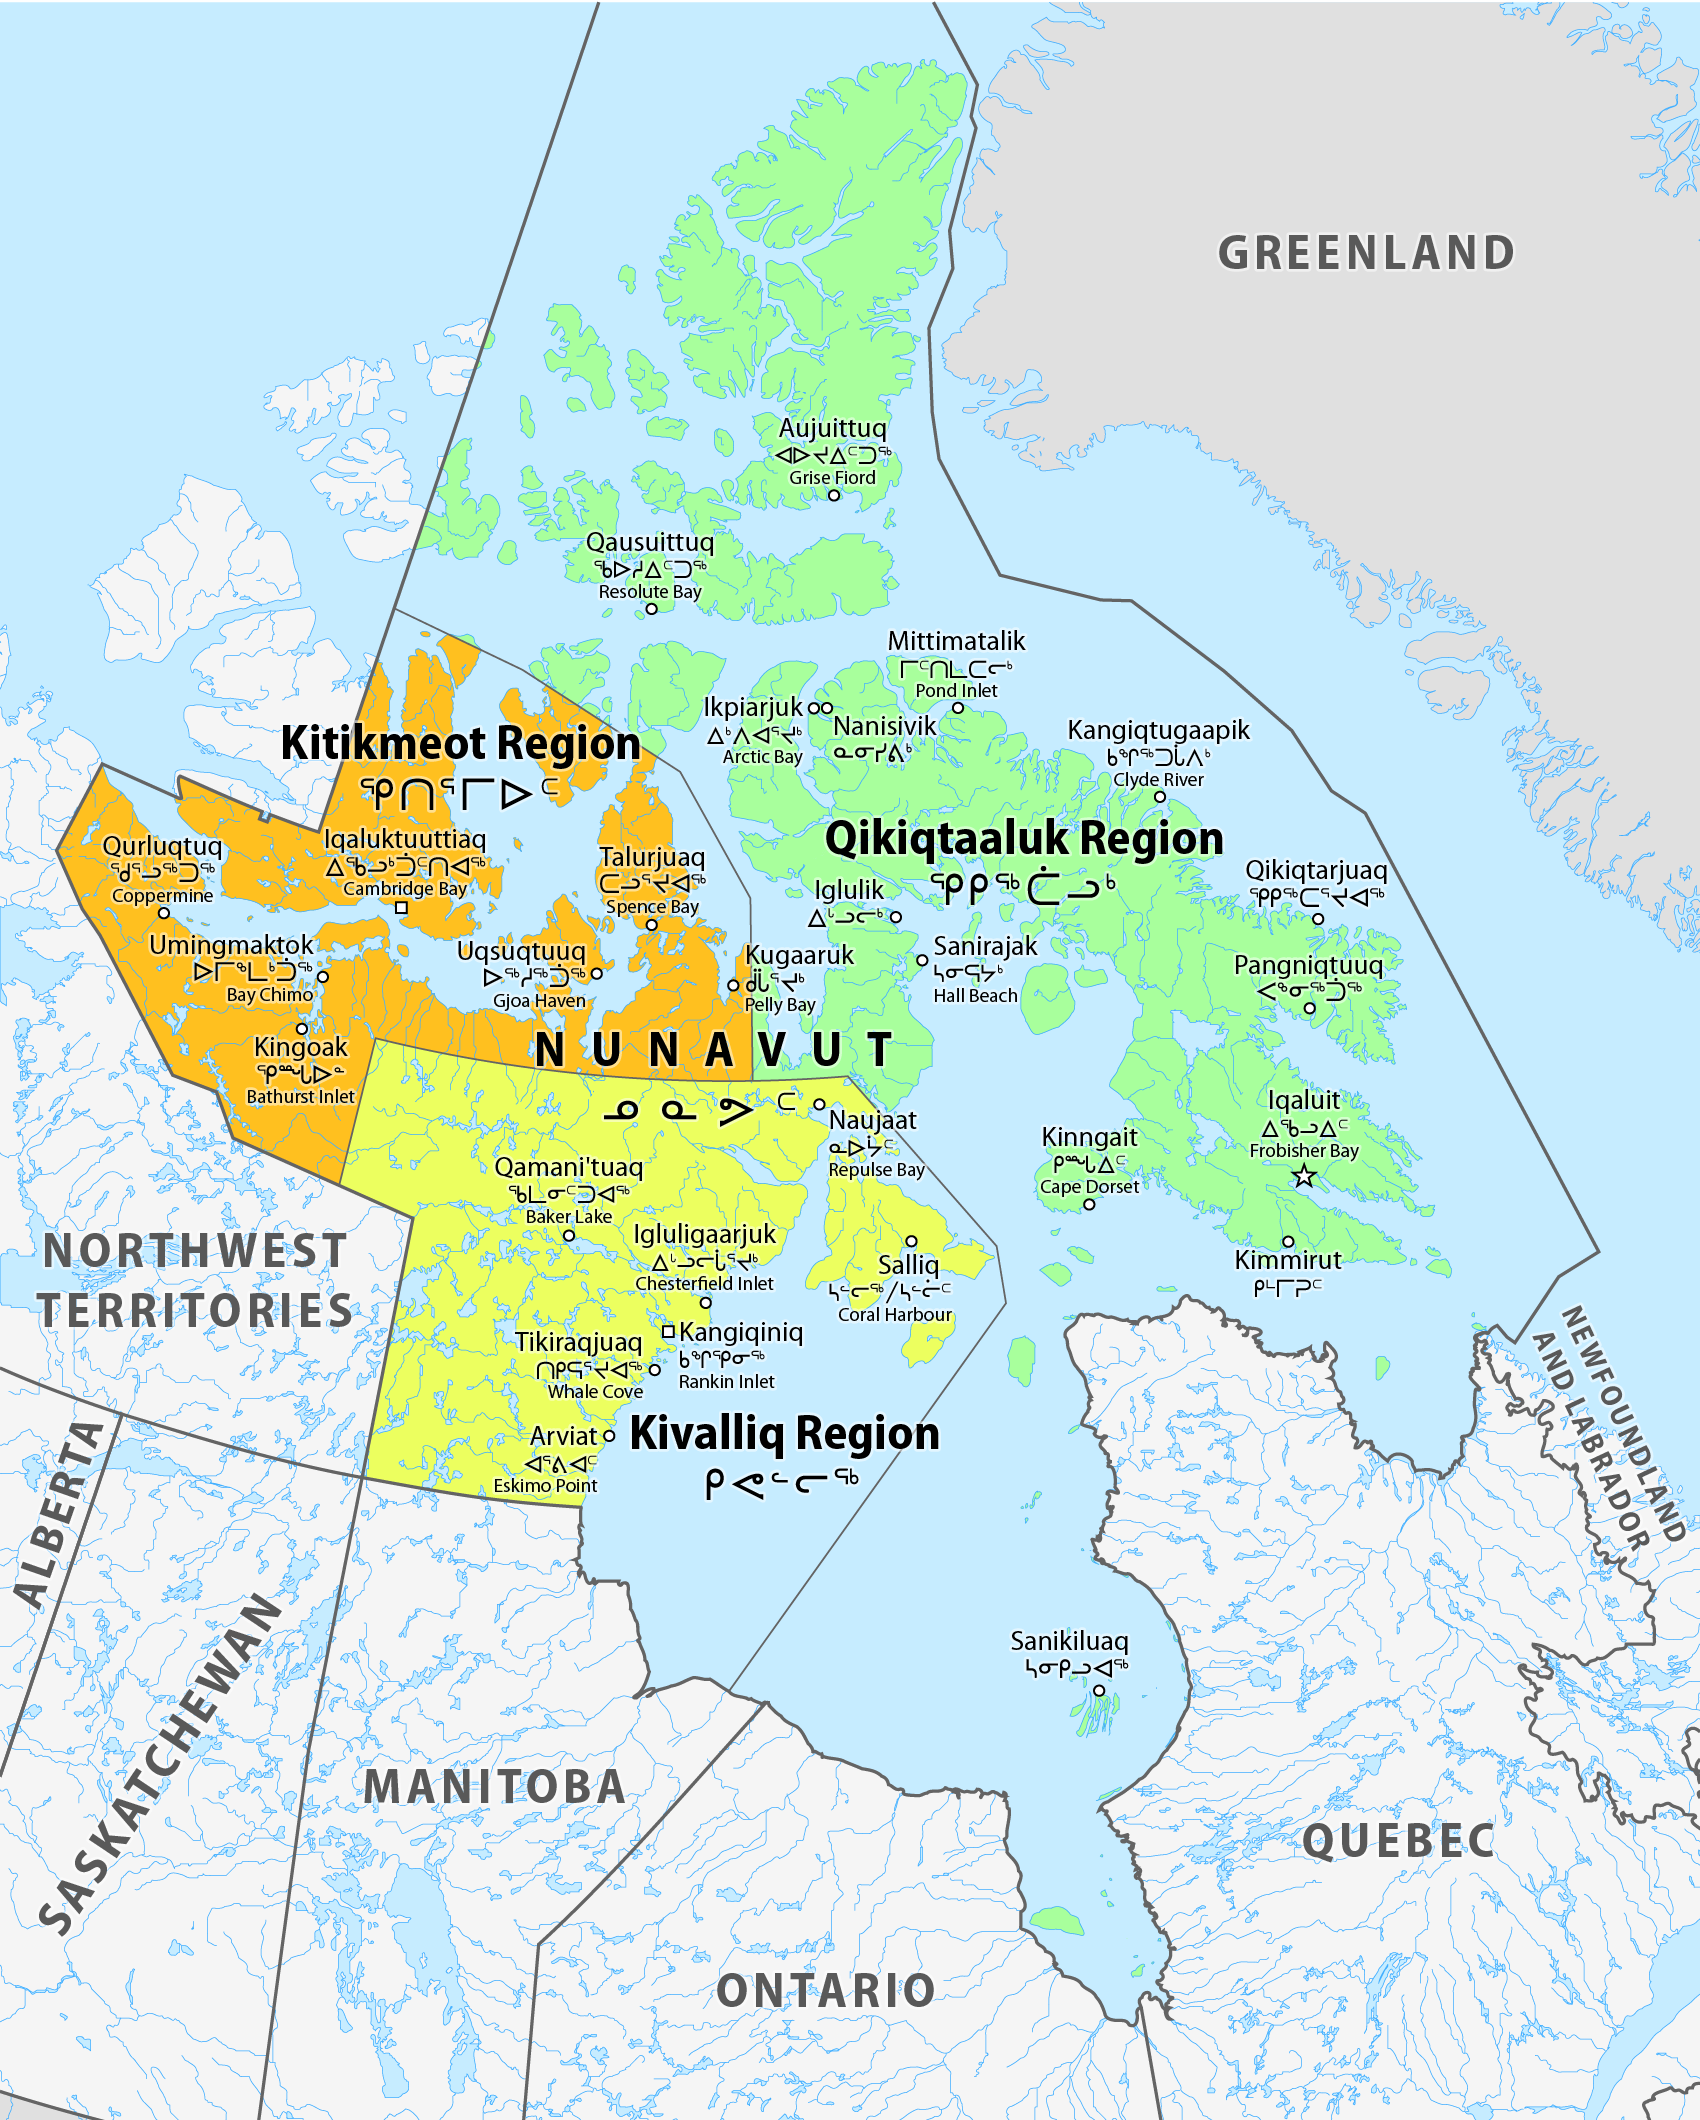
\includegraphics[width = 0.4\textwidth]{Map_Nunavut} & \smash{\raisebox{\height}{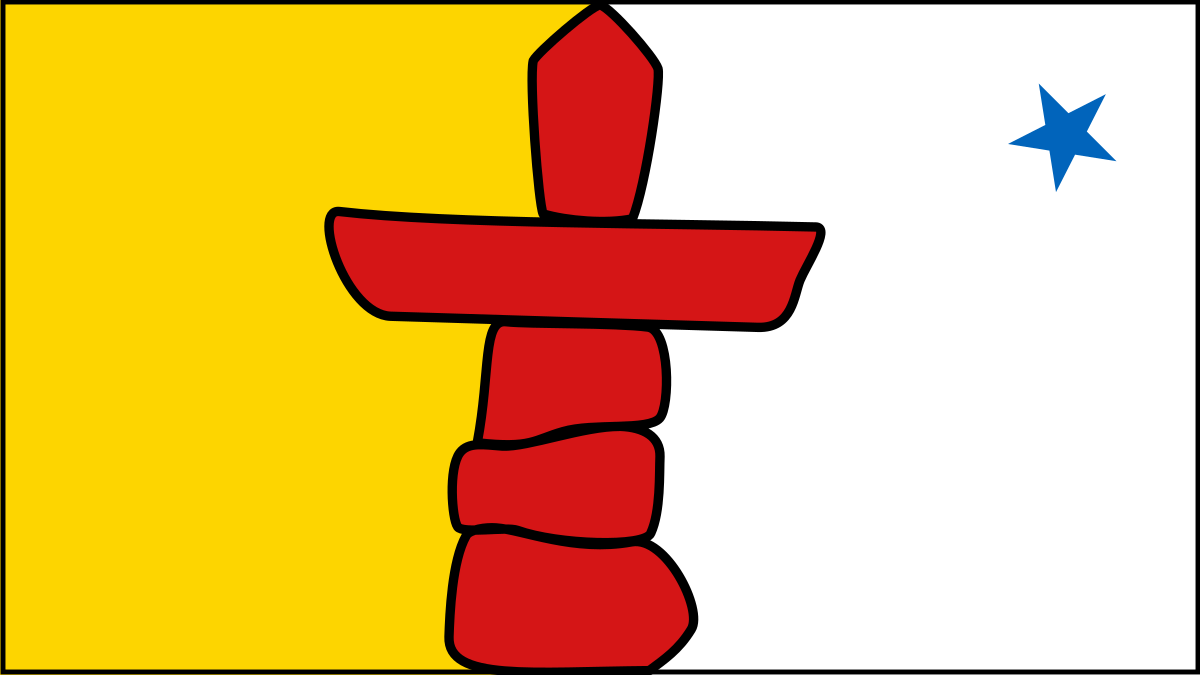
\includegraphics[width = 0.4\textwidth]{Flag_of_Nunavut}}} \\
\end{tabular}
\end{center}

%\begin{center}
%\begin{tabular}{c c}
%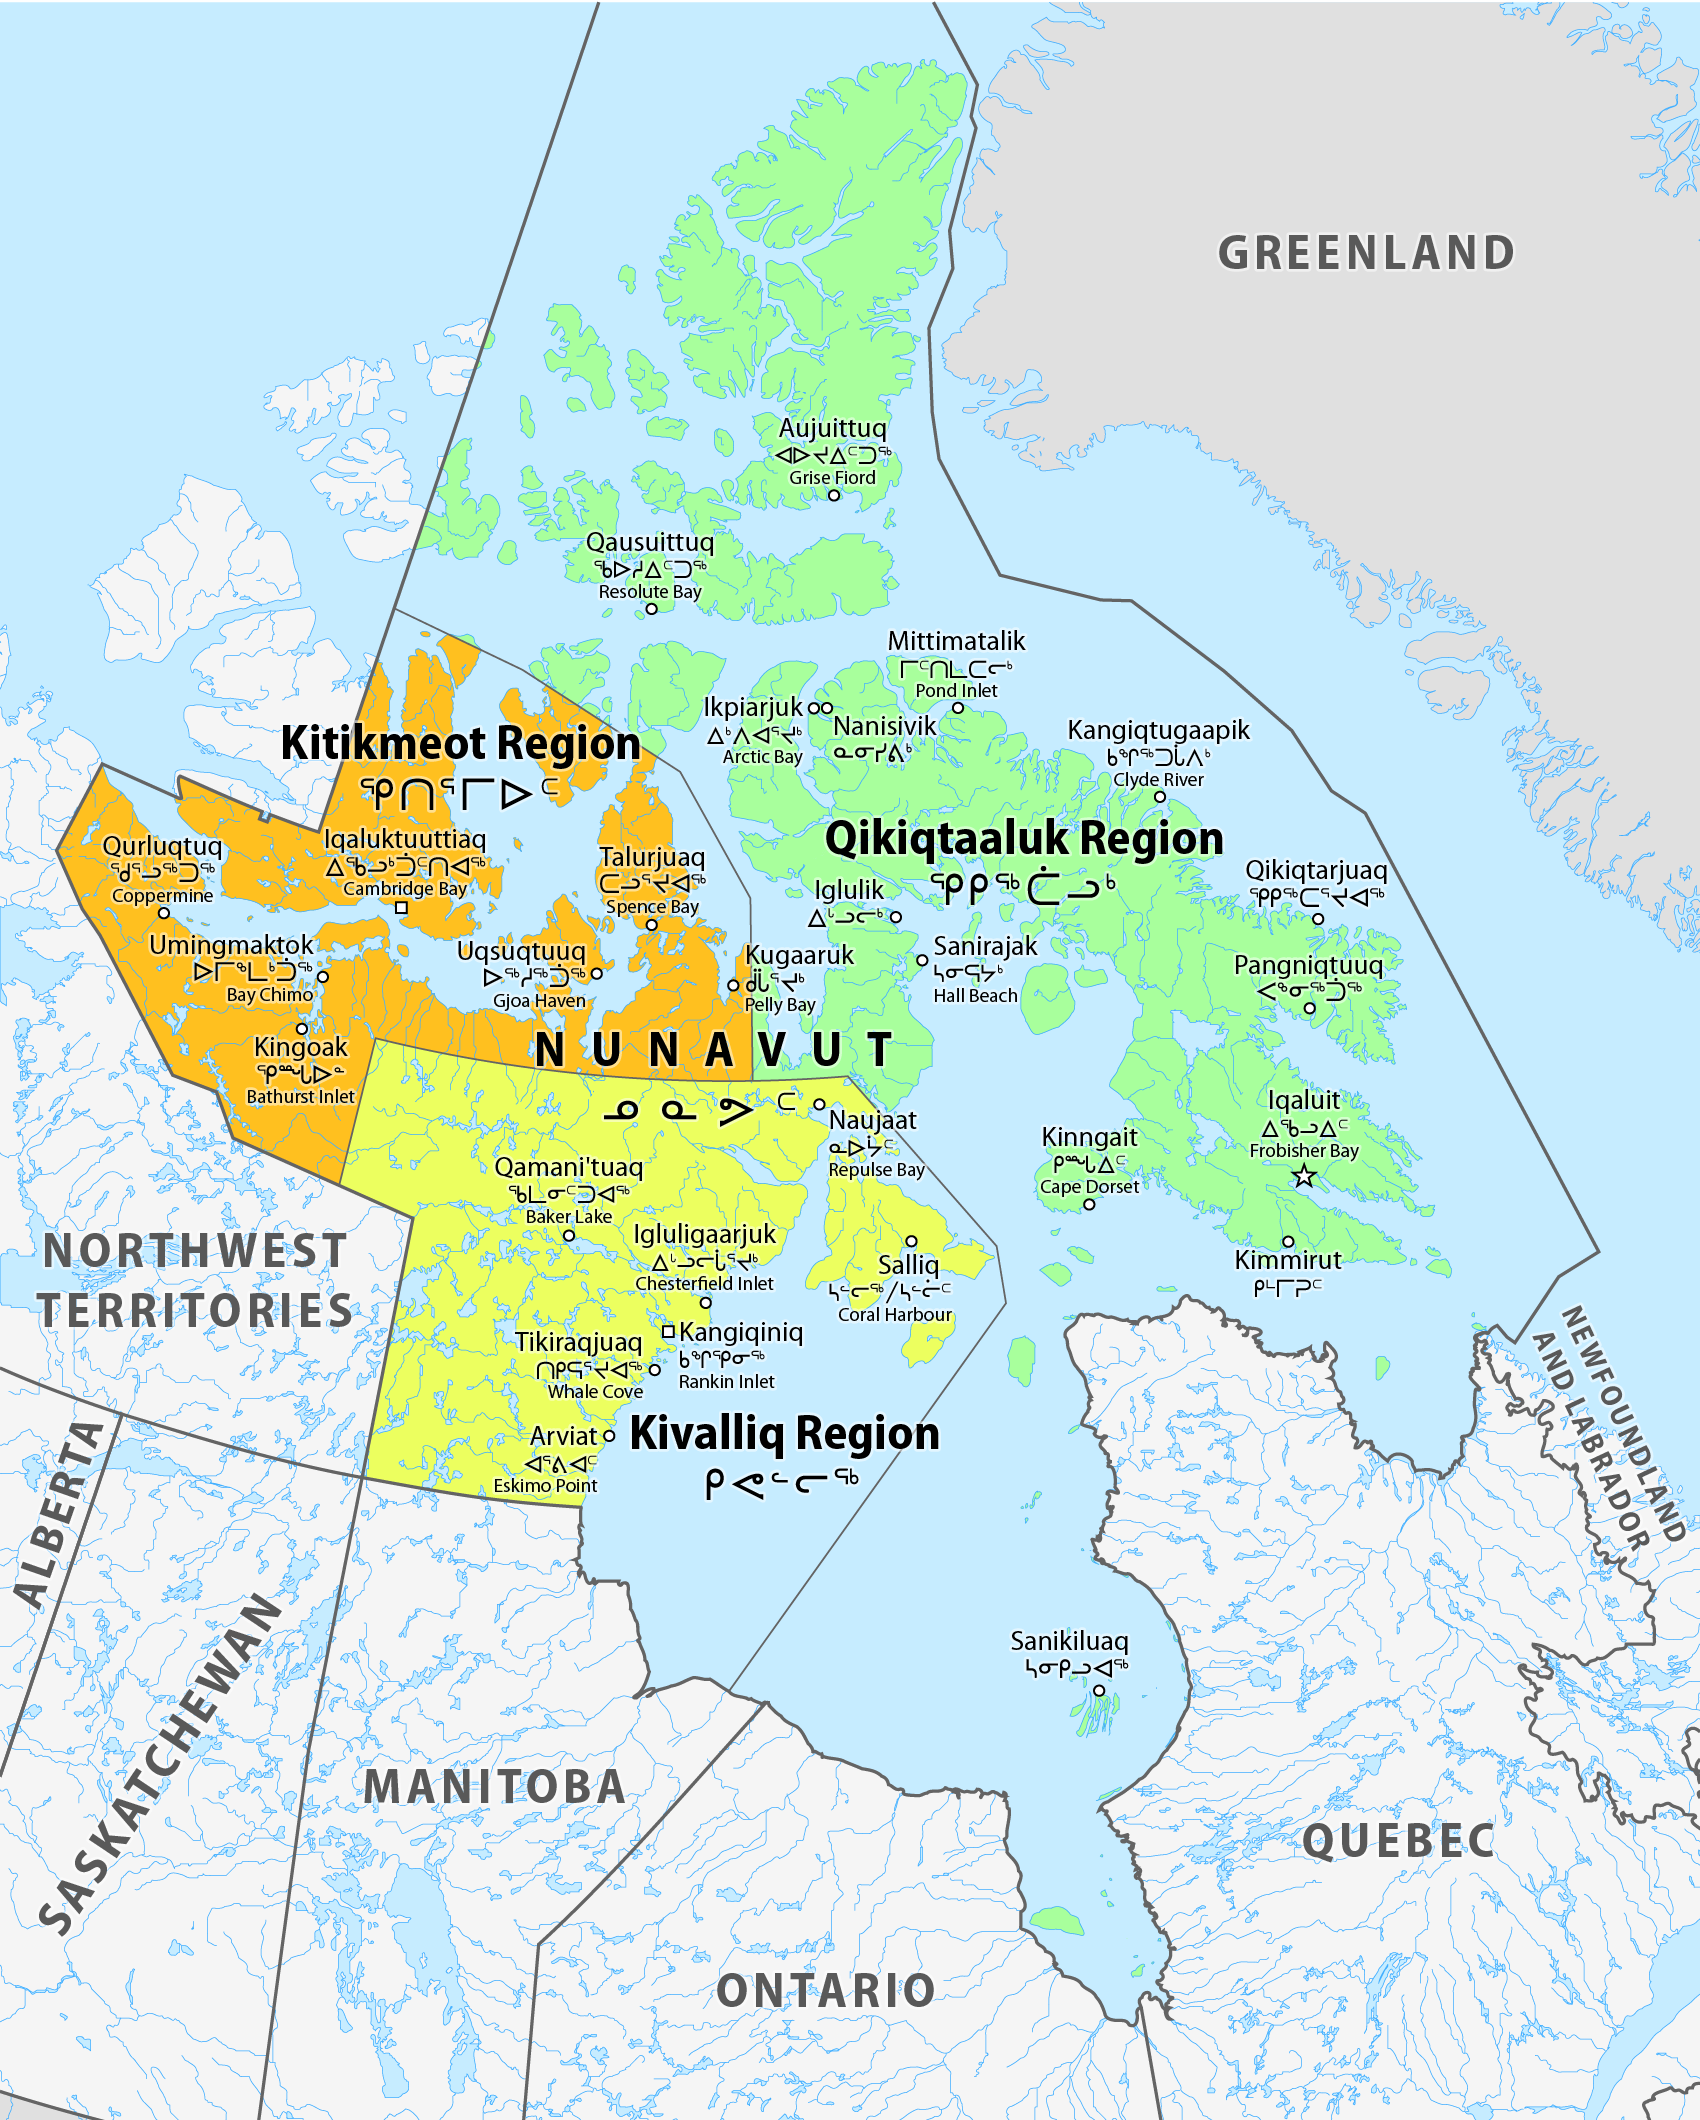
\includegraphics[width = 0.4\textwidth]{Map_Nunavut} & \begin{tabular}[c]{@{}m{18em}@{}} \smash{\raisebox{0.5\height}{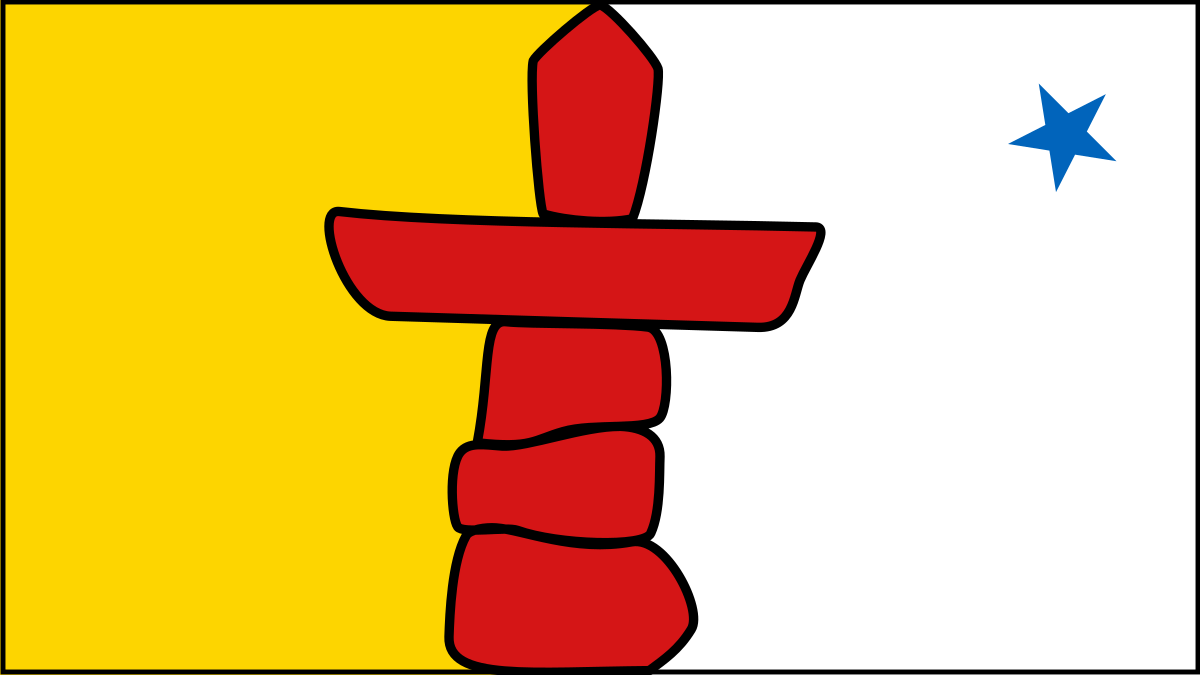
\includegraphics[width = 0.4\textwidth]{Flag_of_Nunavut}}} \\ an \emph{inuksuk} in red is a traditional stone monument used to guide travelers and mark sacred sites; the north star \emph{Niqirtsituk} \\ \end{tabular} \\
%\end{tabular}
%\end{center}


\end{frame}

%%%%%%%%%%%%%%%%%%%%%%%%%%%%%%%%%%%%%%%%%%%%%%%%%%%%%%%%%%%%%%%%%%%%%%

\begin{frame}

The north star also appears in a variety of contexts, from literature, history, religion, and exploration. It also plays an important role in Indigenous and First Nations culture.

\begin{center}
%\begin{tabular}{c c}
%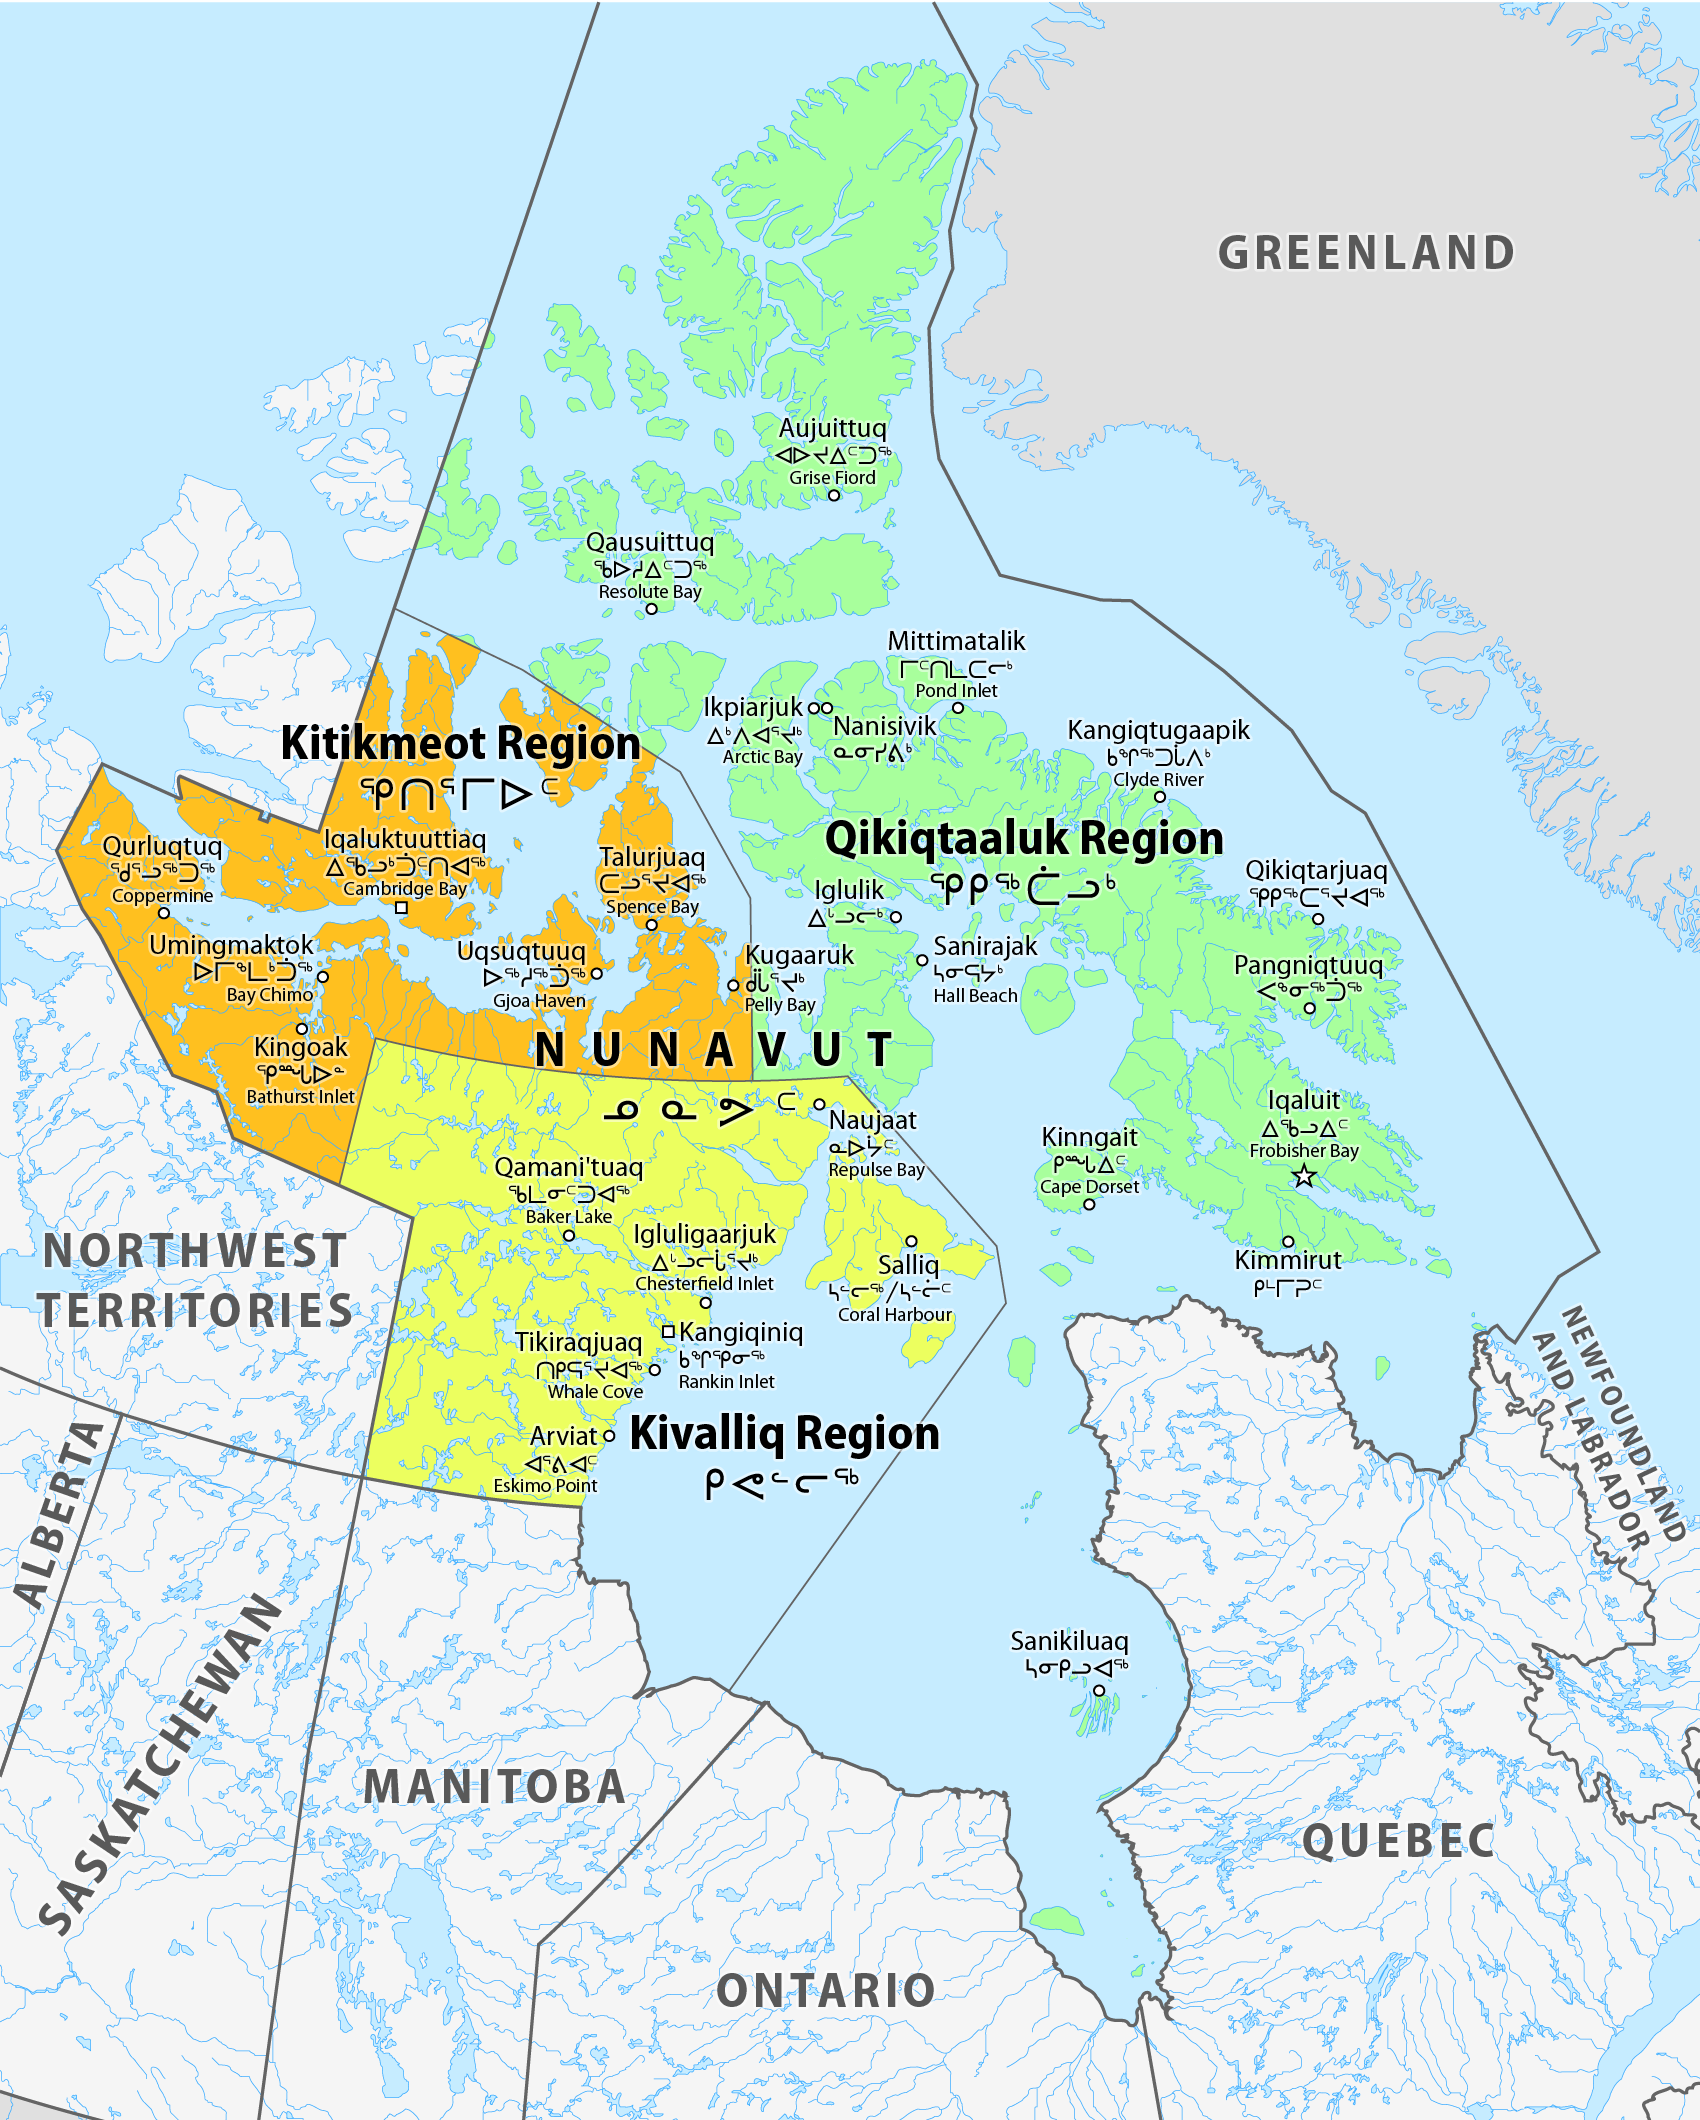
\includegraphics[width = 0.4\textwidth]{Map_Nunavut} &  \begin{tabular}{c} 
\includegraphics[width = 0.4\textwidth]{Flag_of_Alaska} \\ 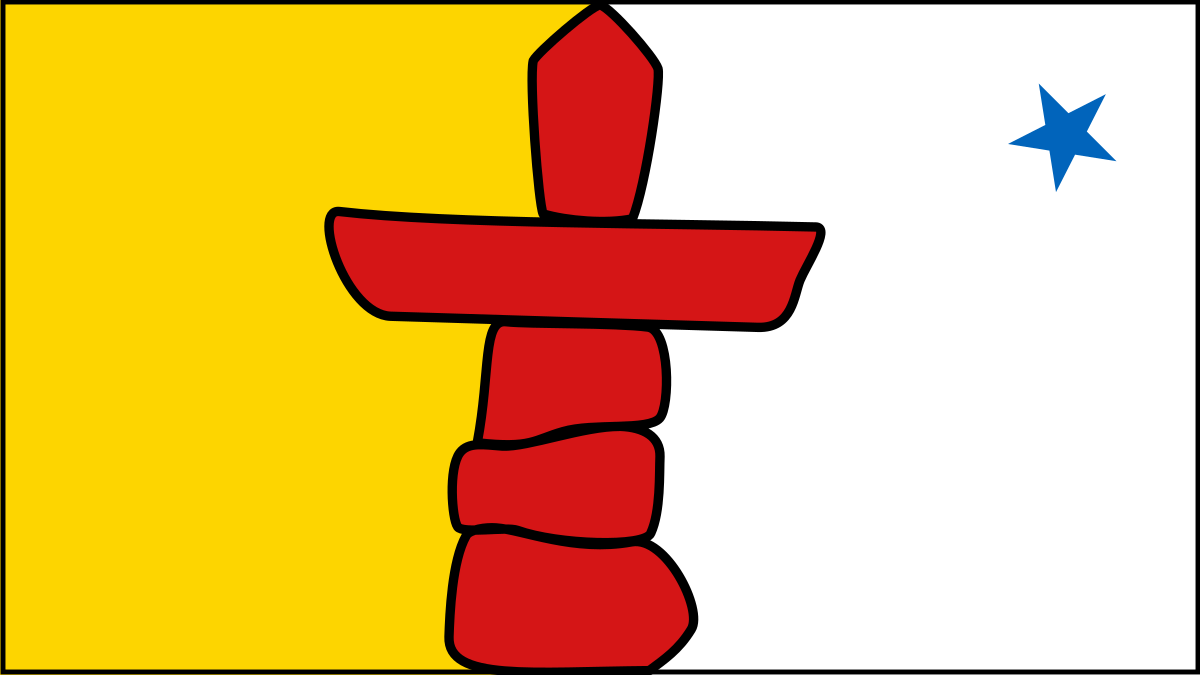
\includegraphics[width = 0.4\textwidth]{Flag_of_Nunavut} \end{tabular}  \\
%\end{tabular}
\begin{tabular}{c c}
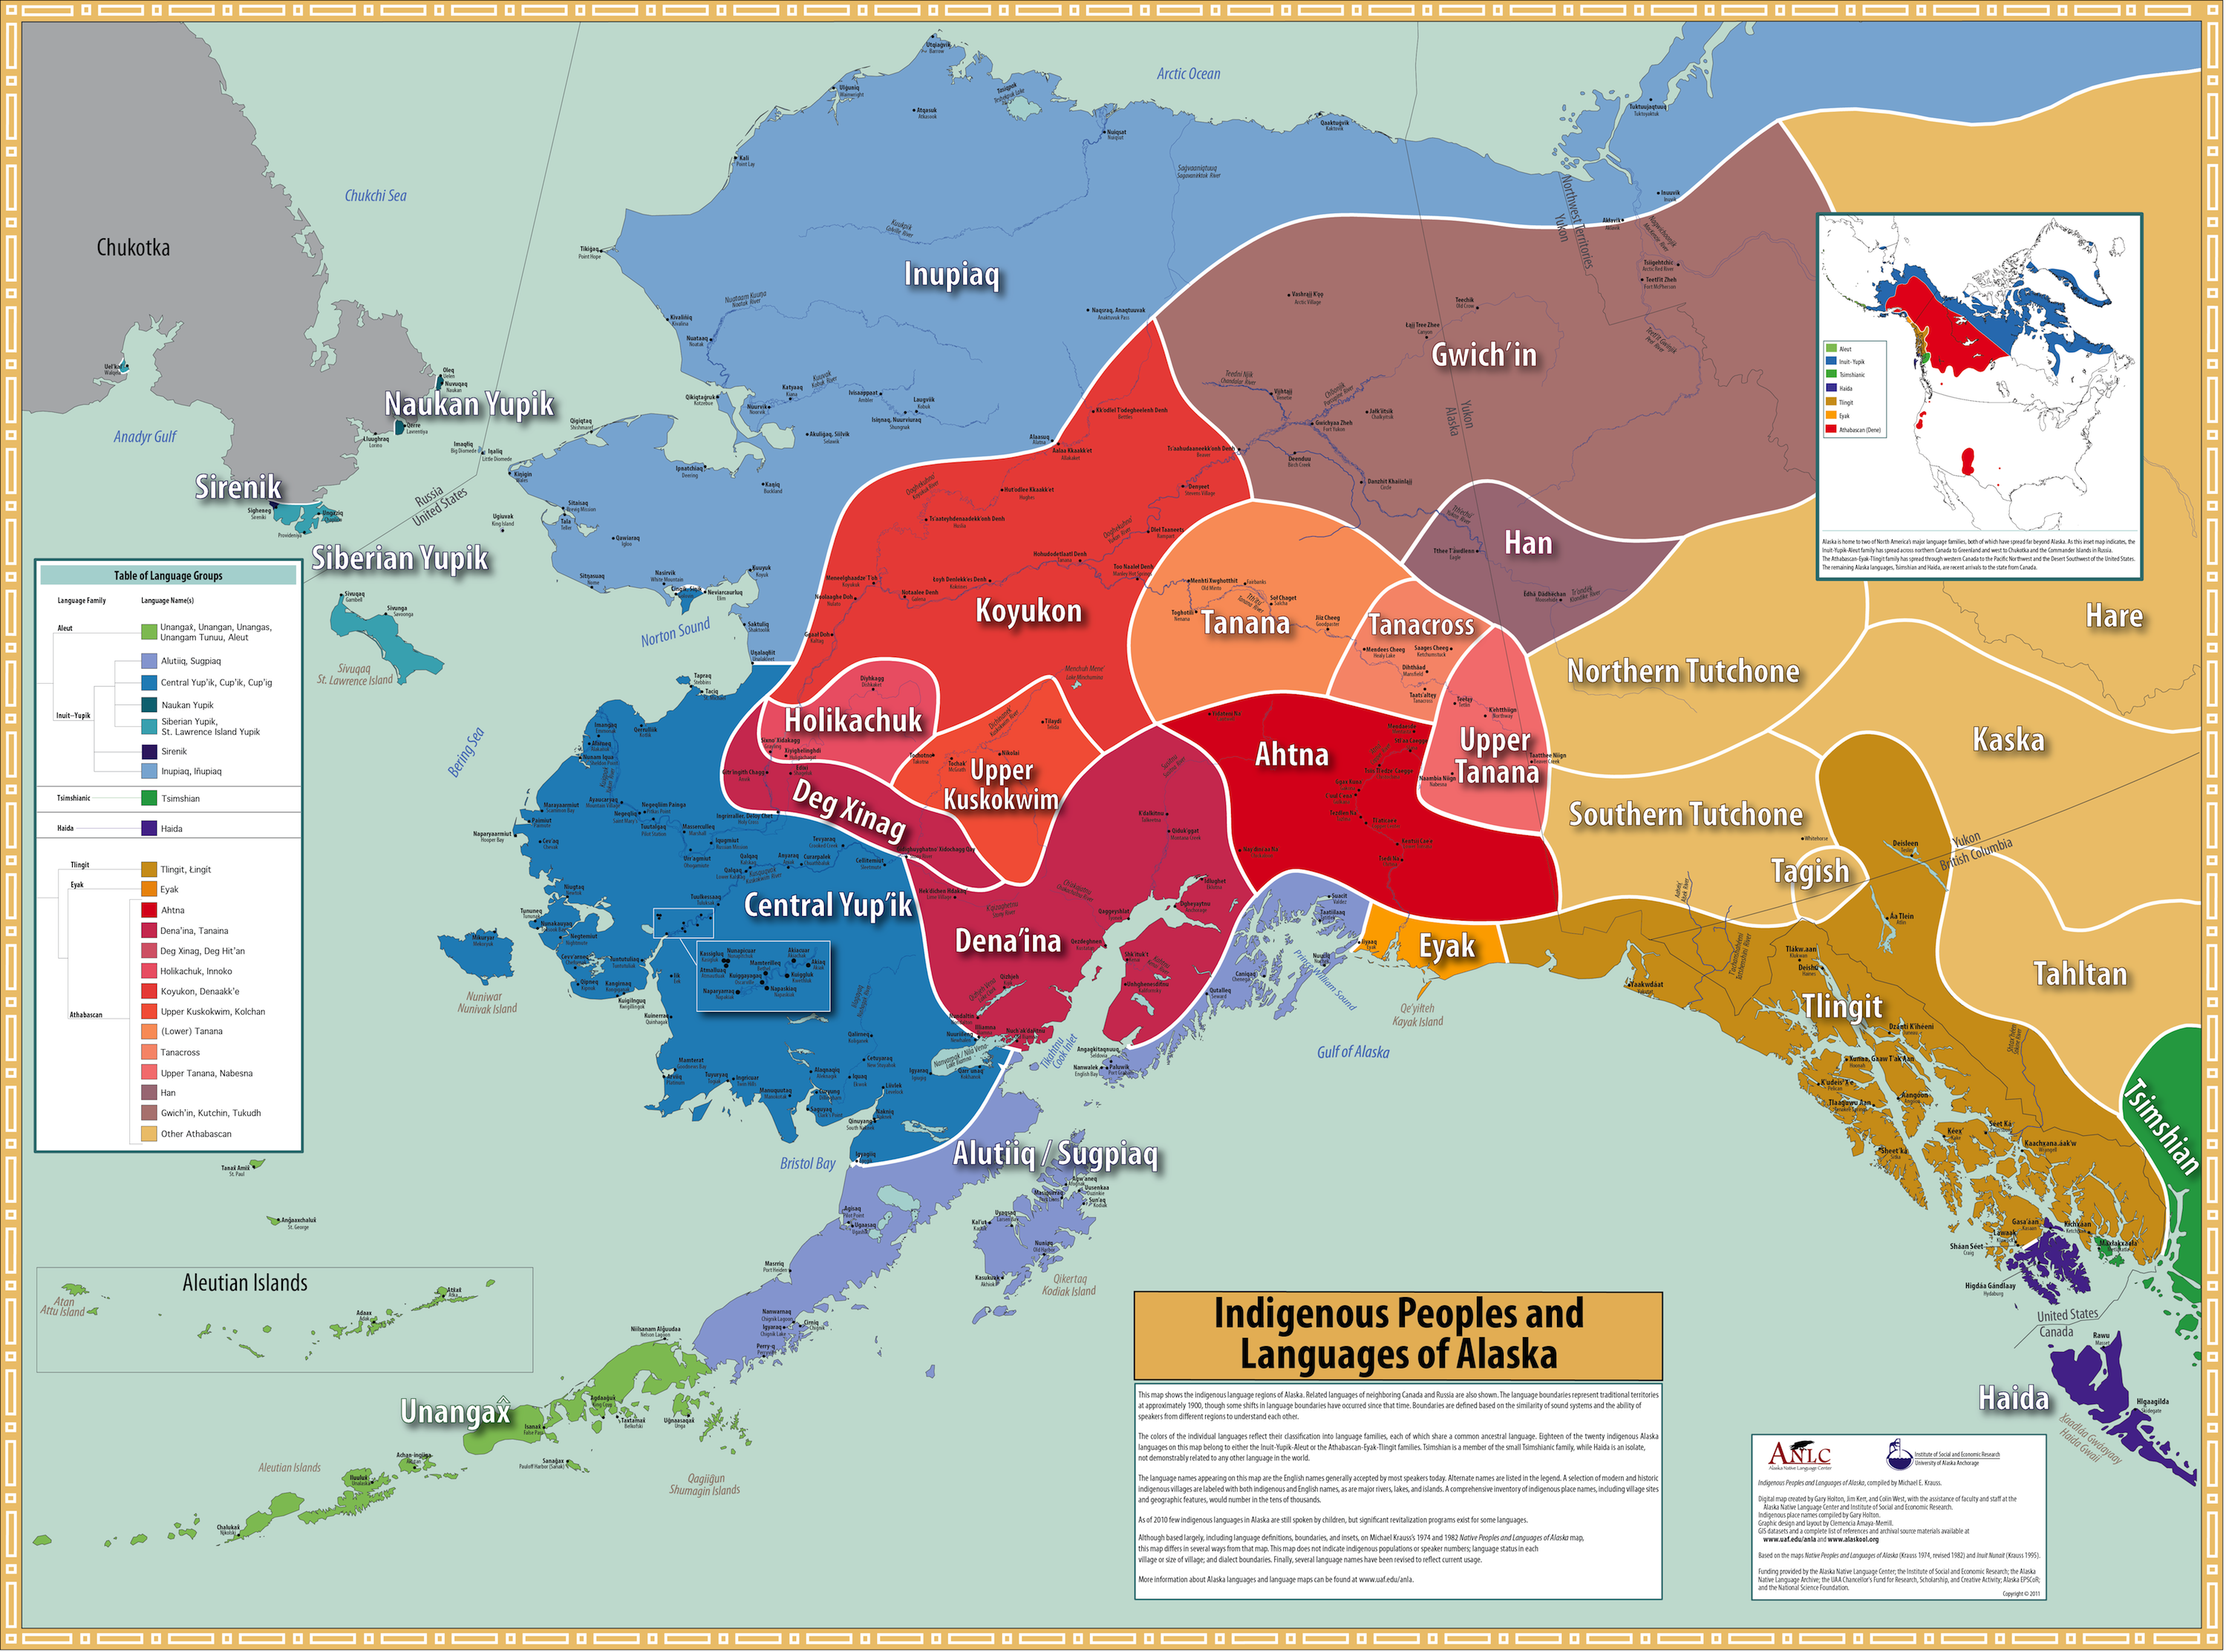
\includegraphics[width = 0.63\textwidth]{anlmap} & \smash{\raisebox{\height}{
\includegraphics[width = 0.3\textwidth]{Flag_of_Alaska}} } \\
\end{tabular}
{\tiny\tt https://www.uaf.edu/anla/collections/map/}
\end{center}

\end{frame}

%%%%%%%%%%%%%%%%%%%%%%%%%%%%%%%%%%%%%%%%%%%%%%%%%%%%%%%%%%%%%%%%%%%%

\begin{frame}

\begin{block}{Problem}
Not everyone lives in the northern hemisphere or close enough to the equator where Polaris is visible. For those in the southern hemisphere, there's a literal planet in the way between you and the north star!

\end{block}

\end{frame}

%%%%%%%%%%%%%%%%%%%%%%%%%%%%%%%%%%%%%%%%%%%%%%%%%%%%%%%%%%%%%%%%%%%%

\begin{frame}

\begin{block}{Flags of the southern hemisphere}
\begin{center}
\begin{tabular}{cc}

\includegraphics[width = 0.4\textwidth]{Flag_of_Australia} & 
\includegraphics[width = 0.4\textwidth]{Flag_of_New_Zealand} \\
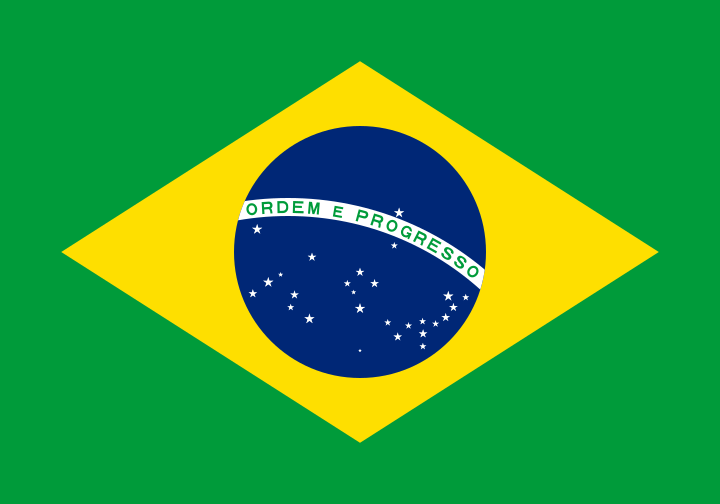
\includegraphics[width = 0.4\textwidth]{Flag_of_Brazil} & 
\includegraphics[width = 0.4\textwidth]{Flag_of_Samoa}
\end{tabular}
\end{center}
\end{block}

\end{frame}

%%%%%%%%%%%%%%%%%%%%%%%%%%%%%%%%%%%%%%%%%%%%%%%%%%%%%%%%%%

\begin{frame}

\vfill

All of these flags share the same constellation, called the Southern Cross (or Crux).

\vfill

\begin{center}
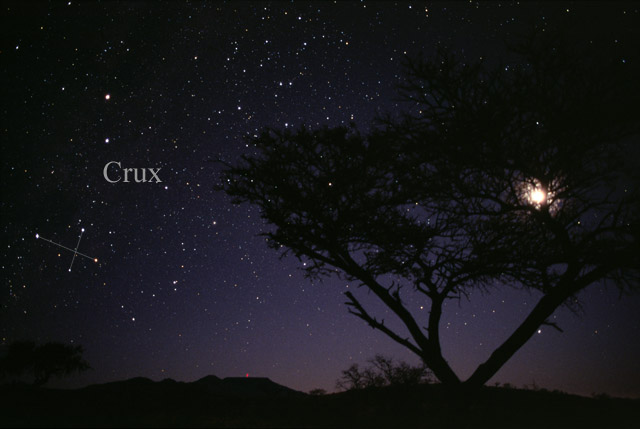
\includegraphics[width=0.6\textwidth]{Constellation_Crux} 
\end{center}

\vfill

\end{frame}

%%%%%%%%%%%%%%%%%%%%%%%%%%%%%%%%%%%%%%%%%%%%%%%%%%%%%%%%%%

\begin{frame}

\vfill

\begin{block}{Application of Geometry \#1}
Use the Southern Cross (and the two pointer stars) to help us find which direction is south:
\end{block}
%\vfill

\begin{center}
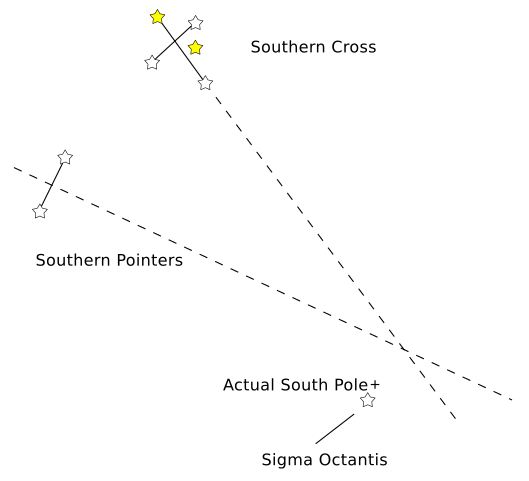
\includegraphics[width=0.55\textwidth]{Navigate_South} 
\end{center}

%\end{block}

\vfill


\end{frame}

%%%%%%%%%%%%%%%%%%%%%%%%%%%%%%%%%%%%%%%%%%%%%%%%%%%%%%%%%

\begin{frame}

\vfill 

\begin{center}
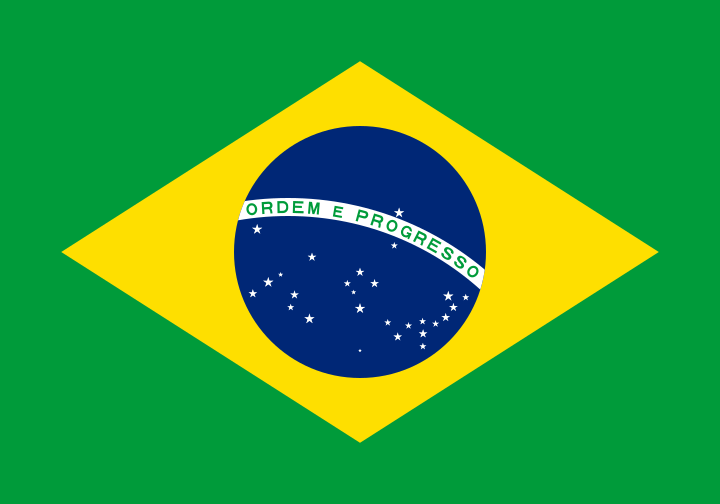
\includegraphics[width=0.7\textwidth]{Flag_of_Brazil} 
\end{center}
{\tiny ``The constellations that figure in the National Flag match the aspect of the sky, in the city of Rio de Janeiro, at 8 hours and 30 minutes of November 15th of 1889 (12 sidereal hours) and must be considered as viewed by an observer outside the celestial sphere." -- Brazilian law on the flag. This is why the Southern Cross is reversed!}

\vfill

\end{frame}

%%%%%%%%%%%%%%%%%%%%%%%%%%%%%%%%%%%%%%%%%%%%%%%%%%%%%%%%%%

\section{Mathematical Billiards}
\begin{frame}
  \sectionpage
\end{frame}

\begin{frame}

\emph{Mathematical billiards} is a dynamical system consisting of a planar connected set $\Omega$ (the \emph{billiard table}) and a point-mass in its interior (the \emph{ball}) which moves in a straight line at constant speed. 

\vskip10pt

%\onslide<2->{When the ball hits the boundary, the ball reflects \emph{elastically}, meaning it follows the rule ``angle of incidence = angle of reflection." }

When the ball hits the boundary, the ball reflects \emph{elastically}, meaning it follows the rule ``angle of incidence = angle of reflection." 

%\vskip10pt

%\onslide<3->{And this process continues. Can we describe the evolution of its dynamics?}

%\vskip10pt

%%works with normal aspect ratio
%\begin{overlayarea}{11cm}{3cm}
%\begin{center}
%\includegraphics<1>[scale=1.5]{BilliardTable1}
%\includegraphics<2>[scale=1.5]{BilliardTable2}
%\includegraphics<3>[scale=1.5]{BilliardTable3}
%\includegraphics<4>[scale=1.5]{BilliardTable4}
%\end{center}
%\end{overlayarea}

\begin{center}
%set up to be used in the 16:9 aspect ratio
\begin{overlayarea}{11cm}{4cm}
\begin{center}
\includegraphics<1>[width=0.75\textwidth]{BilliardTable1a}
\includegraphics<2>[width=0.75\textwidth]{BilliardTable2a}
\includegraphics<3>[width=0.75\textwidth]{BilliardTable3a}
\includegraphics<4>[width=0.75\textwidth]{BilliardTable4a}
\end{center}
\end{overlayarea}
\end{center}

%%\begin{center}
%%%set up to be used in the 16:9 aspect ratio
%%\begin{overlayarea}{11cm}{4cm}
%\begin{center}%
%\includegraphics[width=0.4\textwidth]{EllipticalTableSingleImage}%
%\end{center}%
%%\end{overlayarea}
%%\end{center}

%%Only include the statement below if there isn't a separate slide with the reflection rule on a curved boundary
%Use the angle made with the tangent to the boundary at the point of impact. This is now dependent on the chosen metric! Can also describe this reflection law as $v^- = v_t + v_n \mapsto v_t-v_n = v^+$

\end{frame}

%%%%%%%%%%%%%%%%%%%%%%%%%%%%%%%%%%%%%%%%%%%%%%%%%%%%%%%%%%%%%%%%%%%%%

\begin{frame}
The dynamics of billiards is completely determined by the geometry of the table (e.g. its shape)!

\vskip10pt

One can choose tables of different shapes

\begin{center}
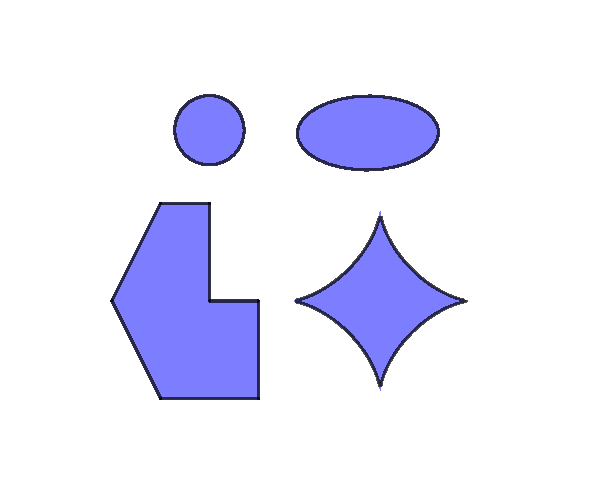
\includegraphics[scale=1.0]{SampleTables}
\end{center}

%One can also assume the billiard table $\Omega$ is in a Riemannian manifold with boundary and the billiard motion will correspond to the geodesic flow. 
\end{frame}

%%%%%%%%%%%%%%%%%%%%%%%%%%%%%%%%%%%%%%%%%%%%%%%%%%%%%%%%%%%%%%%%%%%%%%

\begin{frame}
If the boundary of the table is not a straight line, we need to more accurately describe the reflection law:

%\vskip0.25cm

\begin{center}
\begin{overlayarea}{7cm}{4.5cm}
%\begin{center}
\includegraphics<1>[width=\textwidth]{EllipticalTable1a}
\includegraphics<2>[width=\textwidth]{EllipticalTable2a}
\includegraphics<3>[width=\textwidth]{EllipticalTable3a}
\includegraphics<4->[width=\textwidth]{EllipticalTable4a}
%\end{center}
\end{overlayarea}
\end{center}
\onslide<3->{\textcolor{red}{New reflection law}: use the angle made with the tangent to the boundary at the point of impact.} %\onslide<4->{This is now dependent on the chosen metric!} \\
\onslide<4->{Can also describe this reflection law as $v^- = v_t + v_n \mapsto v_t-v_n = v^+$}
\end{frame}

%%%%%%%%%%%%%%%%%%%%%%%%%%%%%%%%%%%%%%%%%%%%%%%%%%%%%%%%%%%%%%%%%%%%%%

\begin{frame}
These are just several types of planar billiards that are studied:

\begin{table}[b]
\centering
\resizebox{\textwidth}{!}{
\begin{tabular}{l b{9.5cm}}
 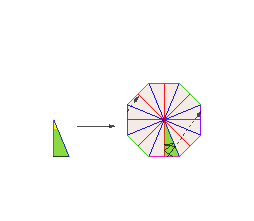
\includegraphics[scale=1.25]{PolygonalBilliard00} & \textcolor<2->{gray}{\emph{Polygonal billiards:} \newline -Related to the study of geodesic flow on a translation surface (with singular points) \newline -Teichm\"{u}ller theory}  \\
& \\
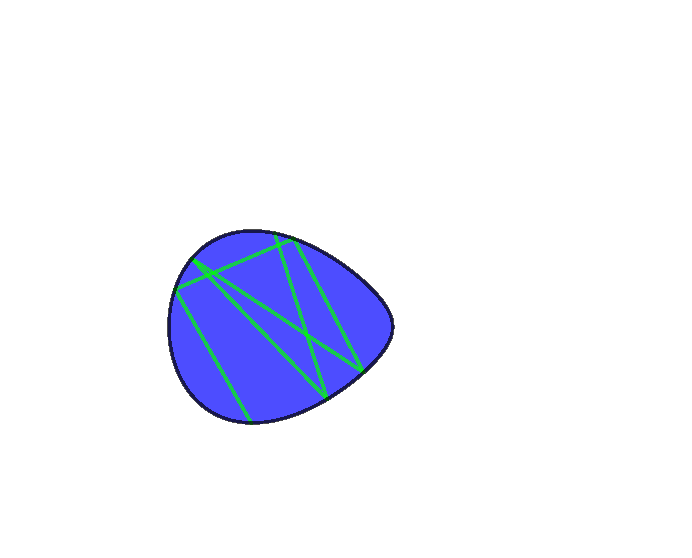
\includegraphics[scale=0.55]{ConvexTable} & \emph{(Strictly) Convex billiards:} \newline -Birkhoff billiards (G. Birkhoff, 1927 - pragmatic example of Hamiltonian systems) \newline -The billiard map is a \emph{twist map} \newline -Coexistence of regular (KAM, Aubry-Mather) and chaotic dynamics \\
 & \\
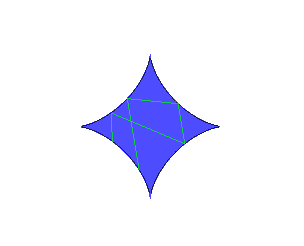
\includegraphics[scale=0.7]{DispersiveBilliard} & \textcolor<2->{gray}{\emph{Concave (or dispersive) billiards:} \newline -Nearby orbits tend to move apart (exponentially) \newline -Hyperbolicity and chaotic behaviour (Sinai, 1970) \newline -Study of statistical properties of orbits}
\end{tabular}
}
\end{table}


\end{frame}

%%%%%%%%%%%%%%%%%%%%%%%%%%%%%%%%%%%%%%%%%%%%%%%%%%%%%%%%%%%%%%%%%%
% 
%\section{Convex Billiards}
%\subsection{}

%%%%%%%%%%%%%%%%%%%%%%%%%%%%%%%%%%%%%%%%%%%%%%%%%%%%%%%%%%%%%%%%%%%%

\begin{frame}
\frametitle{Introduction to Birkhoff Billiards}

Let $\Omega \subset \mathbb{R}^{2}$ be a strictly convex domain with smooth boundary $\partial\Omega$. Fix an orientation of the boundary and measure the angle $\theta_i$ with respect to the positive tangent at the point $p_i$. Parametrize $\partial \Omega = \Gamma$ by arc length $s$ so that the billiard map is 
$$T: \partial \Omega \times (0,\pi) \longrightarrow \partial \Omega \times (0,\pi)$$ $$\;\;\;\;\;\;\;\;(s_i,\theta_i) \longrightarrow (s_{i+1},\theta_{i+1})$$

\vskip5pt

\begin{center}
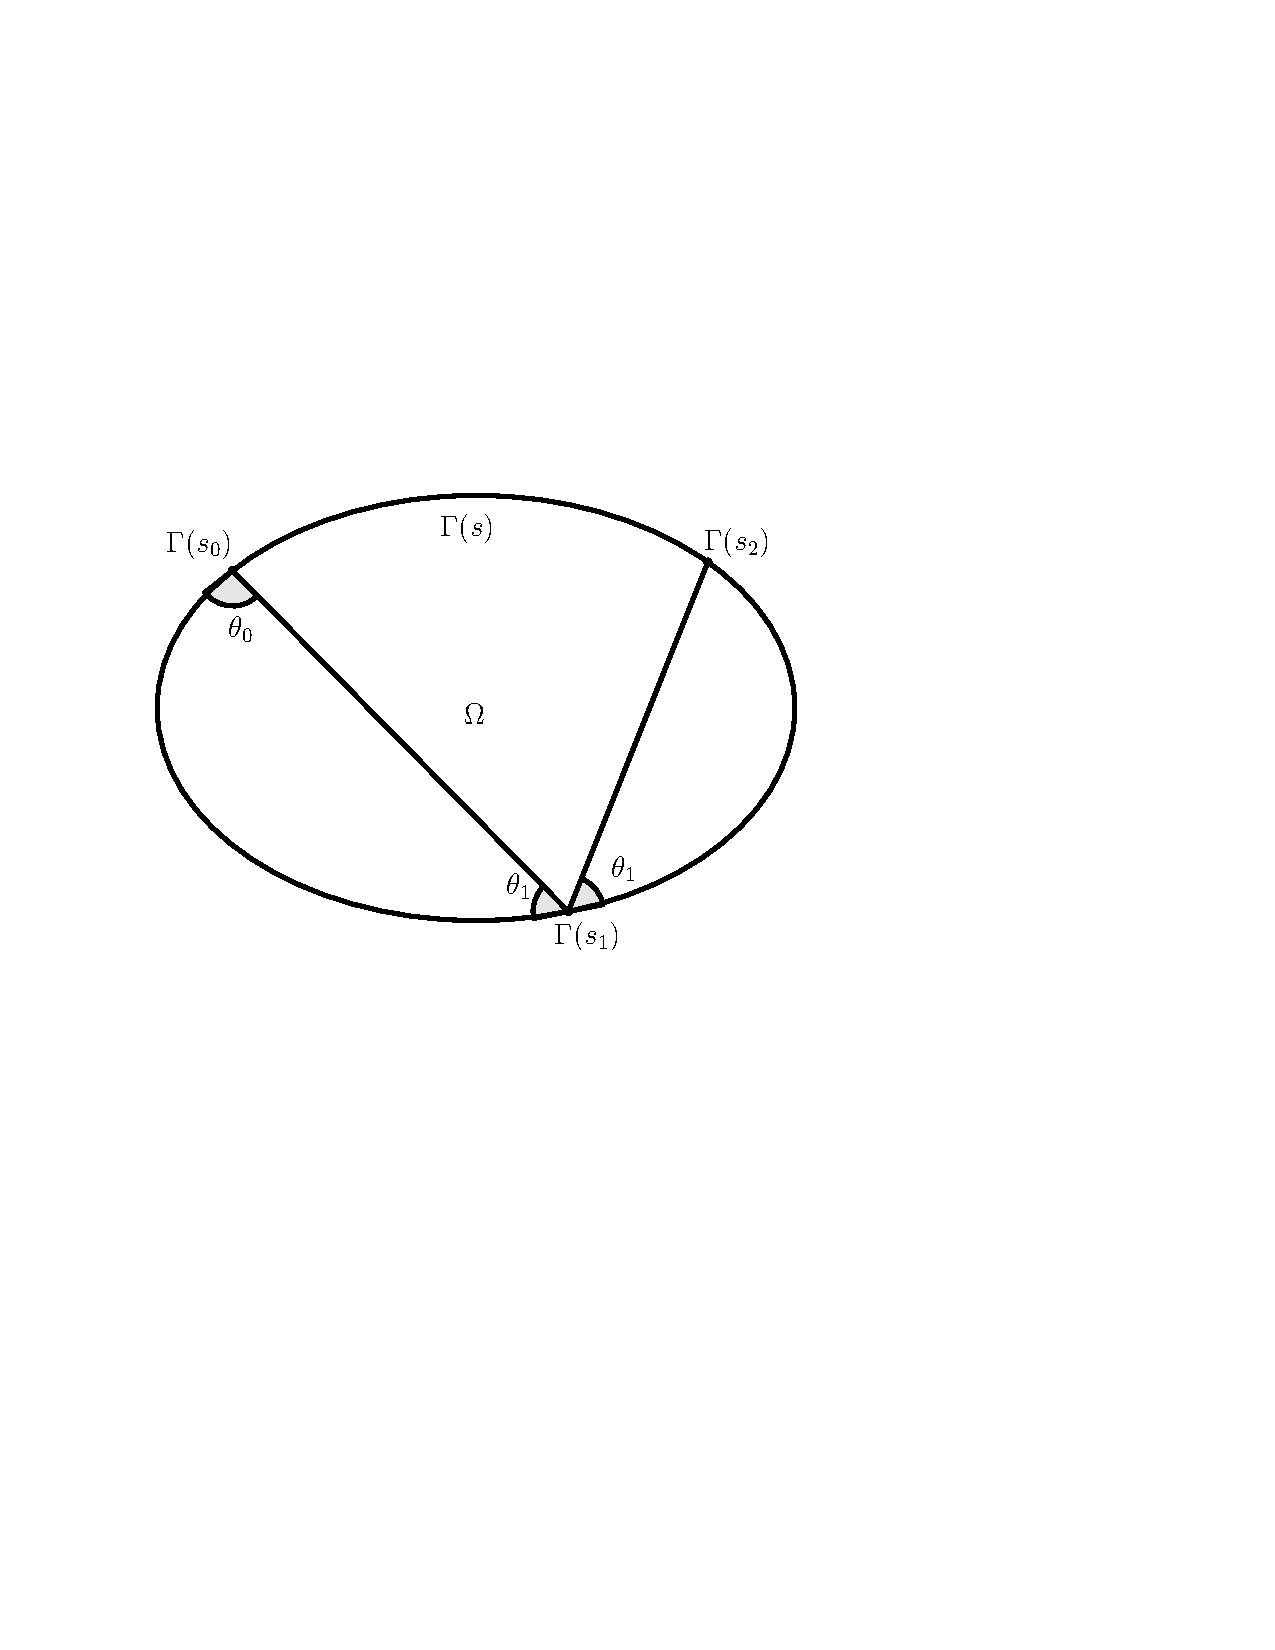
\includegraphics[width = 0.38\textwidth]{BilliardMap}
\end{center}

\end{frame}

%%%%%%%%%%%%%%%%%%%%%%%%%%%%%%%%%%%%%%%%%%%%%%%%%%%%%%%%%%%%%%%%%

%%%Comment out this picture to include separate Circle example
%\begin{frame}
%
%
%\begin{center}
%\begin{tabular}{c c c}
%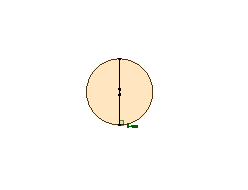
\includegraphics[width=0.25\textwidth]{CirclePeriod2} & 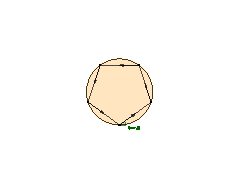
\includegraphics[width=0.25\textwidth]{CirclePeriod5} & \includegraphics[width=0.35\textwidth]{2PeriodBilliardEllipse} \\
%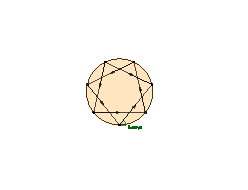
\includegraphics[width=0.25\textwidth]{CirclePeriod7} & 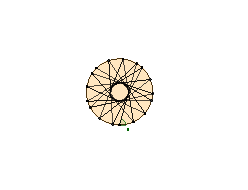
\includegraphics[width=0.25\textwidth]{CircleNPeriodic} & \includegraphics[width=0.35\textwidth]{3PeriodBilliardEllipse}
%\end{tabular}
%\end{center}

%\end{frame}

%%%%%%%%%%%%%%%%%%%%%%%%%%%%%%%%%%%%%%%%%%%%%%%%%%%%%%%%%

%\begin{frame}
%\begin{columns}
%\column{0.50\textwidth}
%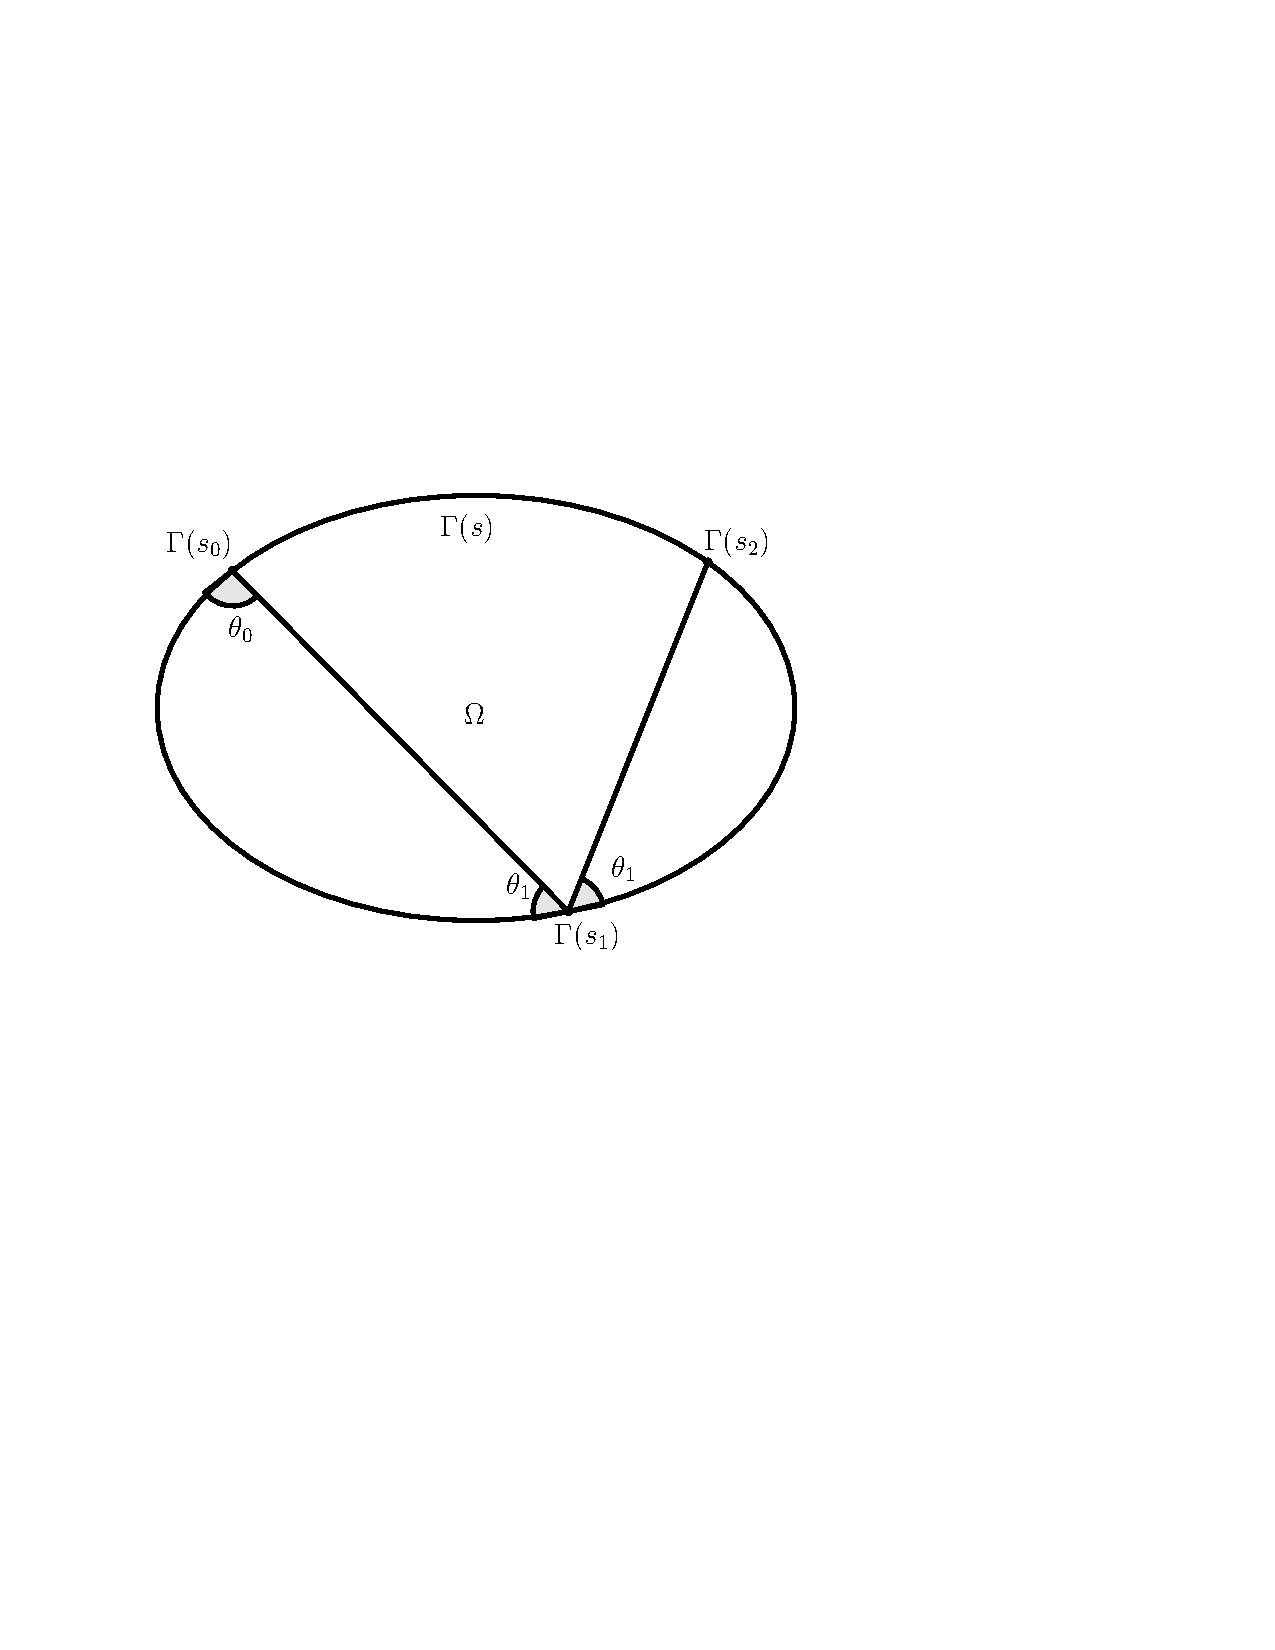
\includegraphics[width = \textwidth]{BilliardMap}
%
%\column{0.50\textwidth}
%\begin{itemize}
%\item<1> Parametrize $\partial \Omega = \Gamma$ by arc length $s$; $|\partial \Omega| = L$
%\item<1> $\theta_i$ is angle between $\Gamma^\prime(s_i)$ and inward velocity vector immediately after collision
%\item<1> Define the billiard map $T: (s_i,\theta_i) \mapsto (s_{i+1}, \theta_{i+1})$
%\item<1> Domain is the open annulus $[0,L) \times (0,\pi)$
%\item<1> Extend to closed annulus $[0,L) \times [0,\pi]$ by continuity
%\end{itemize}
%
%\end{columns}
%\end{frame}

%%%%%%%%%%%%%%%%%%%%%%%%%%%%%%%%%%%%%%%%%%%%%%%%%%%%%%%%%

%\begin{frame}
%\textbf{Properties of the billiard map $T$:}
%\begin{itemize}
%\item $T$ is $C^{r-1}(\mathbb{R}/L\mathbb{Z} \times (0,\pi))$ 
%\item $T$ can be extended continuously to the boundary of the annulus $\mathbb{R}/L\mathbb{Z} \times (0,\pi)$: $T(\cdot,0) = T(\cdot,\pi) = Id$
%\item $T$ is symplectic; it preserves the area form $d\omega = \sin(\theta)d\theta \wedge ds$
%\item $T$ is a \emph{twist map} (applications to KAM theory and Aubry-Mather theory)
%\item $T$ has a generating function $$h(s_i,s_{i+1}) := - \| \Gamma(s_{i+1})-\Gamma(s_i)\|$$ where $\| \cdot\|$ is the Euclidean distance. In particular, this means that $$ 
%\begin{cases}
%\frac{\partial h}{\partial s_i} & = \cos(\theta_i) \\
%\frac{\partial h}{\partial s_{i+1}} & = -\cos(\theta_{i+1}).
%\end{cases}$$
%\end{itemize}
%
%\end{frame}


%%%%%%%%%%%%%%%%%%%%%%%%%%%%%%%%%%%%%%%%%%%%%%%%%%%%%%%%%

\begin{frame}
\begin{example}[Circular Billiard]
\begin{center}
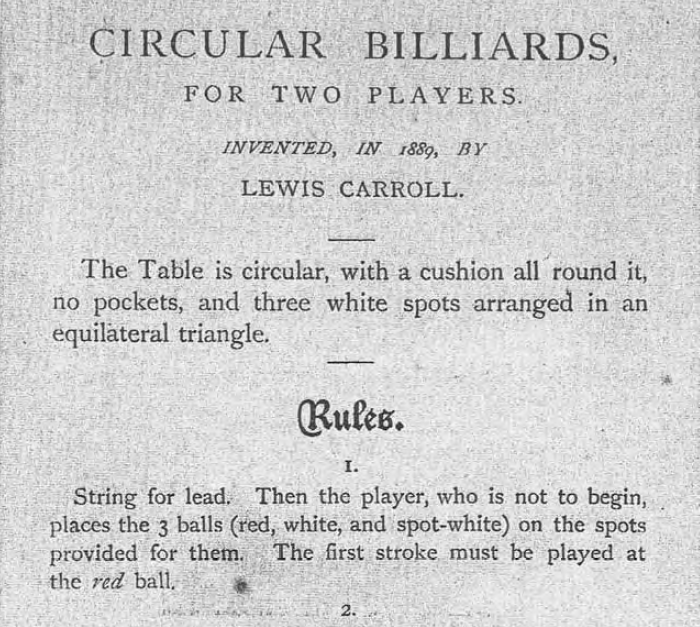
\includegraphics[width=0.60\textwidth]{CircularBilliardRulesCarroll1}
\end{center}
\end{example}

\end{frame}

%%%%%%%%%%%%%%%%%%%%%%%%%%%%%%%%%%%%%%%%%%%%%%%%%%%%%%%%%

\begin{frame}

\begin{center}
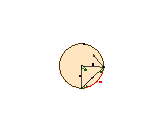
\includegraphics[width=0.4\textwidth]{CircularBilliard}
\end{center}

The map becomes $T(s,\theta) = (s+2R\theta,\theta)$ and the angle $\theta$ is an integral of motion. 

\end{frame}

%%%%%%%%%%%%%%%%%%%%%%%%%%%%%%%%%%%%%%%%%%%%%%%%%%%%%%%%%%

\begin{frame}
If $\theta$ is a rational multiple of $\pi$, the orbit is periodic:

%%% 2x2 grid of billiards
%\begin{center}
%\begin{tabular}{c c }
%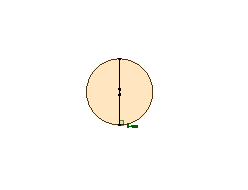
\includegraphics[width=0.22\textwidth]{CirclePeriod2} & 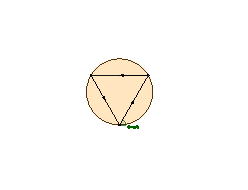
\includegraphics[width=0.22\textwidth]{CirclePeriod3} \\
%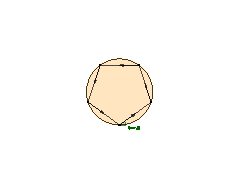
\includegraphics[width=0.22\textwidth]{CirclePeriod5} & 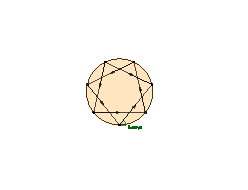
\includegraphics[width=0.22\textwidth]{CirclePeriod7}    
%\end{tabular}
%\end{center}

%%%1x4 grid of billiards
\begin{center}
\begin{tabular}{c c c c}
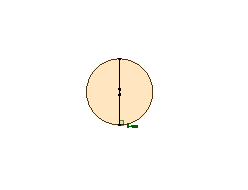
\includegraphics[width=0.22\textwidth]{CirclePeriod2} & 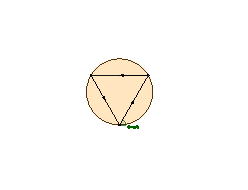
\includegraphics[width=0.22\textwidth]{CirclePeriod3} & 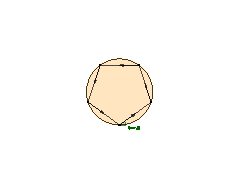
\includegraphics[width=0.22\textwidth]{CirclePeriod5} & 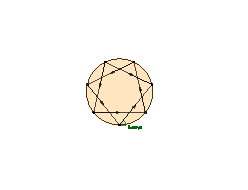
\includegraphics[width=0.22\textwidth]{CirclePeriod7}    
\end{tabular}
\end{center}

For every $p/q \in (0,1/2]$ there exist \emph{infinitely many} periodic orbits which bounce $q$ times (\emph{period}) and turn $p$ times around the circle (\emph{winding number}) before closing. We call $p/q$ the \emph{rotation number}. 

\end{frame}

%%%%%%%%%%%%%%%%%%%%%%%%%%%%%%%%%%%%%%%%%%%%%%%%%%%%%%%%

\begin{frame}

If $\theta$ is not a rational multiple of $\pi$ then the trajectory hits the boundary at a dense set of points.

\begin{center}
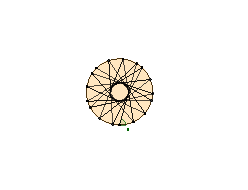
\includegraphics[width=0.35\textwidth]{CircleNPeriodic}
\end{center}

The trajectory is always tangent to a circle (an example of a \emph{caustic}).

\end{frame}

%%%%%%%%%%%%%%%%%%%%%%%%%%%%%%%%%%%%%%%%%%%%%%%%%%%%%%%%%

\begin{frame}

\vfill

\begin{definition}
A \emph{caustic} is a curve with the property that each trajectory (or its extension) that is tangent to it stays tangent after each reflection. 
\end{definition}

\vfill

\begin{center}
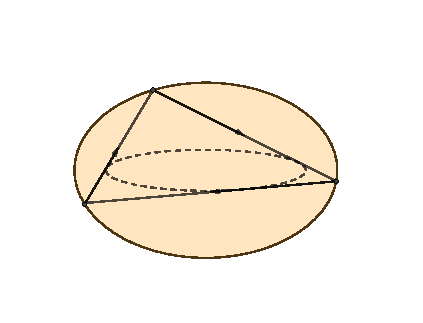
\includegraphics[width=0.4\textwidth]{Caustic}
\end{center}

\vfill

%To a convex caustic in $\Omega$ there is an \emph{invariant circle} of $T$ in phase space. The converse is not necessarily true: invariant circles give rise to caustics but they might not be convex or differentiable. 

\end{frame}

%%%%%%%%%%%%%%%%%%%%%%%%%%%%%%%%%%%%%%%%%%%%%%%%%%%%%%%%%

%\begin{frame}
%
%\begin{block}{Integrability and Billiards}
%There are several ways to define integrability for Hamiltonian systems:
%\begin{itemize}
%\item Liouville-Arnol'd integrability (existence of integrals of motion)
%\item $C^0$-integrability (existence of a foliation by invariant Lagrangian submanifolds)
%\end{itemize}
%\end{block}
%
%\begin{center}
%Integrability $\iff$ (part of) the billiard table is foliated by caustics.
%\end{center}
%
%\vskip10pt
%
%\onslide<2->{
%\begin{center}
%\includegraphics[width = 0.4\textwidth]{CirclePS} \\
%Phase space of the billiard in a circle
%\end{center}}
%
%\end{frame}

%%%%%%%%%%%%%%%%%%%%%%%%%%%%%%%%%%%%%%%%%%%%%%%%%%%%%%%%

%\begin{frame}
%\textbf{(Non?)Existence of Caustics}
%\begin{itemize}
%\item Do there exist examples of billiards with at least one caustic? \begin{itemize}\item Yes! By means of the string construction:\newline  \begin{center} \includegraphics[width=0.5\textwidth]{StringConstruction} \end{center} \end{itemize}
%\item Do there exist examples of billiards with infinitely many caustics? \begin{itemize}\item
%Yes! Lazutkin (1973) proved that via a coordinate change every Birkhoff billiard is \emph{nearly integrable} using a KAM-type theorem: a Cantor set of caustics accumulate near the boundary \end{itemize}
%\item Do there exist examples of billiards with no caustics? \begin{itemize}\item Yes! If the curvature of the boundary vanishes then no caustics can accumulate near the boundary (Mather, 1984). \end{itemize}
%%\item Are there other billiards admitting a foliation by caustics?
%\end{itemize}
%
%\end{frame}

%%%%%%%%%%%%%%%%%%%%%%%%%%%%%%%%%%%%%%%%%%%%%%%%%%%%%%%%%

\begin{frame}
\begin{example}[Elliptical Billiard]
\begin{center}
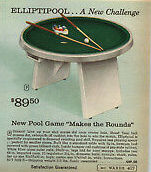
\includegraphics[width=0.35\textwidth]{Elliptipool2}
\end{center}

{\small
The New York Times (1st July 1964) ran a full-page ad for \emph{Elliptipool}, played on an elliptical table with a single pocket at one focus. The ad said that on the following day the game would be demonstrated at Stern's department store by movie stars Paul Newman and Joanne Woodward.
}

\end{example}
\end{frame}

%%%%%%%%%%%%%%%%%%%%%%%%%%%%%%%%%%%%%%%%%%%%%%%%%%%%%%%%%

\begin{frame}
\begin{example}[Elliptical Billiard]
\centering 
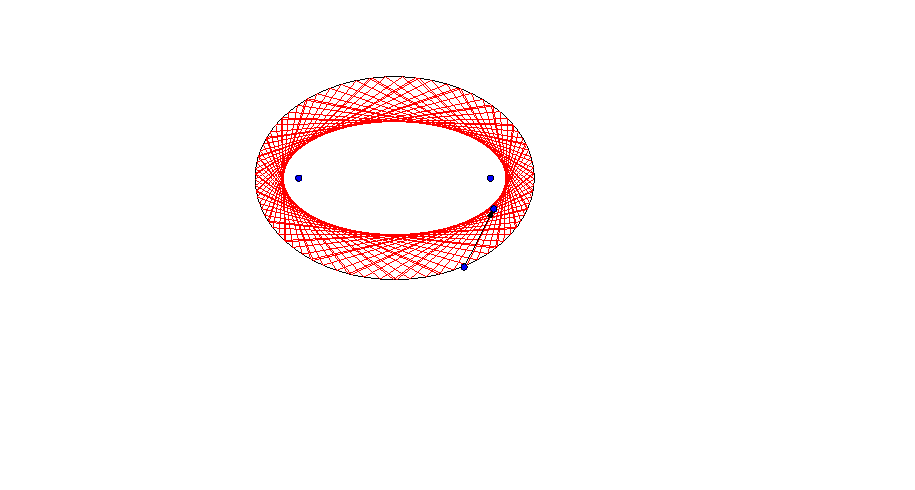
\includegraphics[scale=2.0]{EllBillEll}
\end{example}
\end{frame}


%%%%%%%%%%%%%%%%%%%%%%%%%%%%%%%%%%%%%%%%%%%%%%%%%%%%%%%%%%

\begin{frame}
\centering
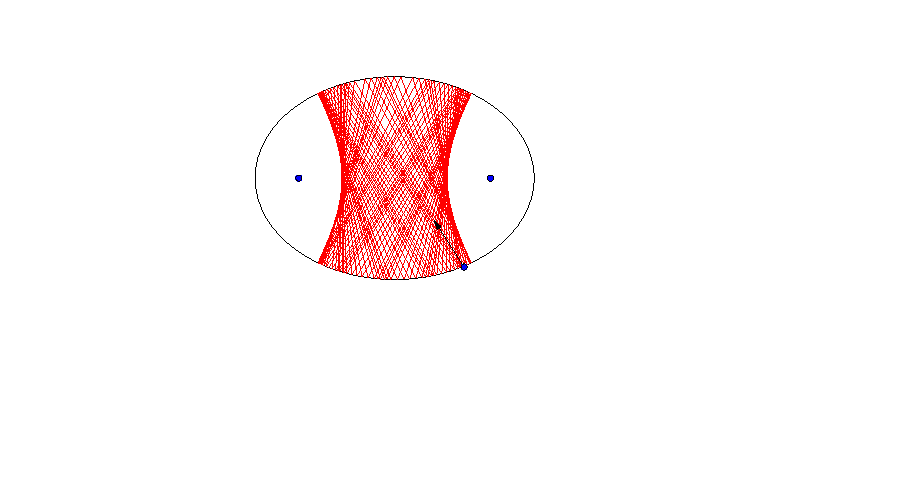
\includegraphics[scale=2.0]{EllBillHyp}
\end{frame}

%%%%%%%%%%%%%%%%%%%%%%%%%%%%%%%%%%%%%%%%%%%%%%%%%%%%%%%%%%

\begin{frame}
\centering
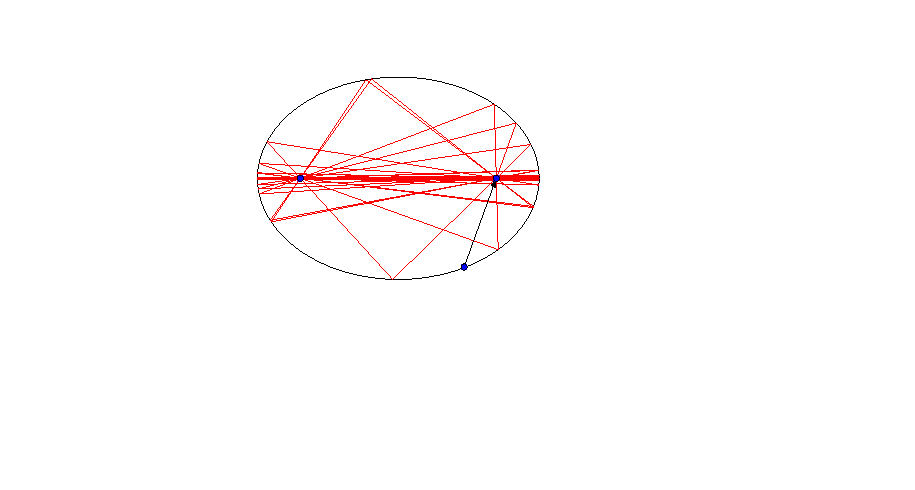
\includegraphics[scale=2.0]{EllBillFoc}
\end{frame}

%%%%%%%%%%%%%%%%%%%%%%%%%%%%%%%%%%%%%%%%%%%%%%%%%%%%%%%%%

\begin{frame}

\begin{block}{Applications of Geometry \#2}
Let's prove some of these properties of elliptical billiards. 
\end{block}

\onslide<2->
Consider a billiard inside the ellipse
$$
\mathcal{E}:\;\;\frac{x^2}{a^2}+\frac{y^2}{b^2}, \quad a > b >0.
$$

\begin{center}
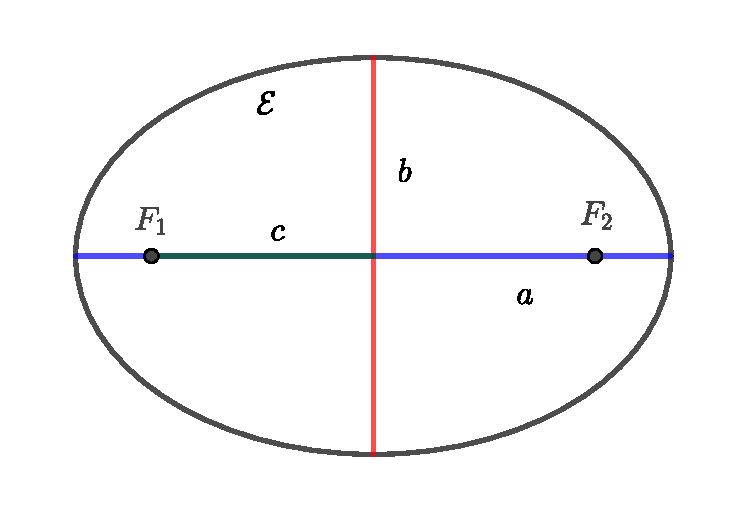
\includegraphics[width=0.45\textwidth]{Ellipse}
\end{center}

The focal distance $c = \sqrt{a^2-b^2}$ and foci are at $F_1 = (-c,0)$ and $F_2 = (c,0)$

\end{frame}

%%%%%%%%%%%%%%%%%%%%%%%%%%%%%%%%%%%%%%%%%%%%%%%%%%%%%%%%%

\begin{frame}

\vfill

\begin{definition}
An ellipse is the closed plane curve such that for all point $P$ on the curve, the sum of the two distances to the focal points is constant. Specifically, $|PF_1| + |PF_2| = 2a$. 
\end{definition}

\vfill

\begin{center}
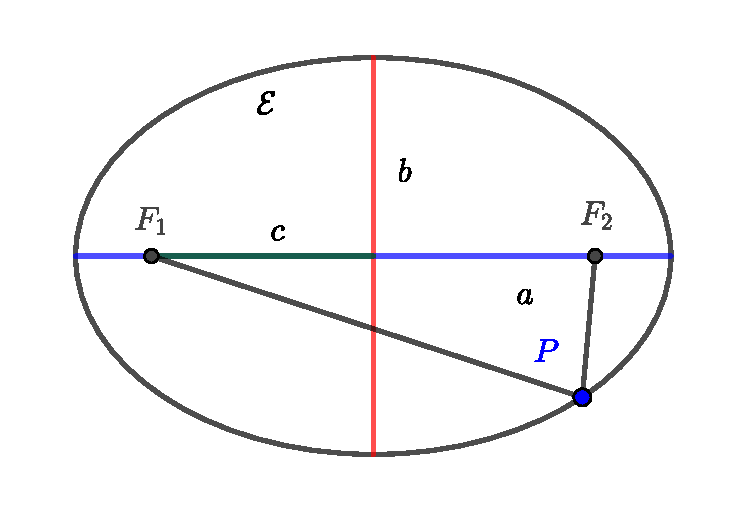
\includegraphics[width=0.5\textwidth]{EllipseAlt}
\end{center}

\vfill

\end{frame}

%%%%%%%%%%%%%%%%%%%%%%%%%%%%%%%%%%%%%%%%%%%%%%%%%%%%%%%%%

\begin{frame}

\vfill

\begin{center}
\includegraphics[width=0.5\textwidth]{EllipseAlt}
\end{center}

\vfill

\begin{block}{Key Observation}
Points inside $\mathcal{E}$ satisfy $|PF_1| + |PF_2| < 2a$ while points outside of $\mathcal{E}$ satisfy $|PF_1| + |PF_2| > 2a$. 
\end{block}

\vfill

\end{frame}

%%%%%%%%%%%%%%%%%%%%%%%%%%%%%%%%%%%%%%%%%%%%%%%%%%%%%%%%%

\begin{frame}

\vfill

\begin{block}{Proposition}
Let $P$ be a point on the ellipse $\mathcal{E}$. The angle bisectors of the lines $\overleftrightarrow{PF_1}$ and $\overleftrightarrow{PF_2}$ are the tangent and normal lines to $\mathcal{E}$ at $P$.  
\end{block}

\vfill

\onslide<2->

\begin{center}
\includegraphics[width=0.5\textwidth]{EllipseProp1WTS}
\end{center}

\vfill


\end{frame}

%%%%%%%%%%%%%%%%%%%%%%%%%%%%%%%%%%%%%%%%%%%%%%%%%%%%%%%%%

\begin{frame}

\vfill

\begin{block}{Proof}
\begin{itemize}
\item Let $\ell$ and $m$ be the angle bisectors of $\overleftrightarrow{PF_1}$ and $\overleftrightarrow{PF_2}$. 
\item By Axiom 7 and Theorem 86, $2(red\; angle) + 2(green \; angle) = 180^\circ$ $\implies$ $(red\; angle) + (green\; angle) = 90^\circ$. So $\ell$ is perpendicular to $m$.
\item This means that if we can show $\ell$ is the tangent line, then $m$ will automatically be the normal line.  
\end{itemize}
\end{block}

\begin{center}
\includegraphics[width=0.4\textwidth]{EllipseProp1A}
\end{center}

\vfill

\end{frame}

%%%%%%%%%%%%%%%%%%%%%%%%%%%%%%%%%%%%%%%%%%%%%%%%%%%%%%%%%

\begin{frame}

\vfill

\begin{block}{Proof (cont.)}
\begin{itemize}
\item Let $R$ be any point on $\ell$ other than $P$. 
\item Construct the line perpendicular to $\ell$ through $F_2$. This line intersects $\ell$ at $Q$ and intersects $\overleftrightarrow{PF_1}$ at $B$. Connect $R$ to $B$ and $R$ to $F_2$. 
\end{itemize}
\end{block}

\begin{center}
\includegraphics[width=0.5\textwidth]{EllipseProp1B}
\end{center}

\vfill

\end{frame}

%%%%%%%%%%%%%%%%%%%%%%%%%%%%%%%%%%%%%%%%%%%%%%%%%%%%%%%%%

\begin{frame}

\vfill

\begin{block}{Proof (cont.)}
\begin{itemize}
\item Since $PQ \cong PQ$, $\Delta PQF_2 \cong \Delta PQB$ by ASA.  
\item By CPCFC, $QF_2 \cong QB$ and $PB \cong PF_2$. This makes $\ell$ the perpendicular bisector of $F_2B$. 
\end{itemize}
\end{block}

\begin{center}
\includegraphics[width=0.5\textwidth]{EllipseProp1C}
\end{center}

\vfill

\end{frame}

%%%%%%%%%%%%%%%%%%%%%%%%%%%%%%%%%%%%%%%%%%%%%%%%%%%%%%%%%

\begin{frame}

\vfill

\begin{block}{Proof (cont.)}
\begin{itemize}
\item Since $RQ \cong RQ$, $\Delta RQF_2 \cong \Delta RQB$ by SAS.  
\item By CPCFC, $RF_2 \cong RB$. 
\item Construct $R F_1$. 
\end{itemize}
\end{block}

\begin{center}
\includegraphics[width=0.4\textwidth]{EllipseProp1D}
\end{center}

\vfill

\end{frame}

%%%%%%%%%%%%%%%%%%%%%%%%%%%%%%%%%%%%%%%%%%%%%%%%%%%%%%%%%

\begin{frame}

\vfill

\begin{block}{Proof (cont.)}
\begin{itemize}
\item Moreover,
$$
|RF_1| + |RF_2| = |RF_1| + |RB| \geq |F_1B| = |PF_1| + |PB| = |PF_1| + |PF_2| = 2a.
$$
\item Therefore $R$ is outside $\mathcal{E}$, and so all points on $\ell$ other than $P$ are outside $\mathcal{E}$. 
\item The inequality is strict unless $R=P$. Therefore $P$ is the only point that $\ell$ shares with $\mathcal{E}$, making $\ell$ the tangent line to $\mathcal{E}$ and $m$ the normal line. \qed
%
%\begin{align*}
%|RF_1| + |RF_2| &= |RF_1| + |RB| \\
%	&> |F_1B| \quad \text{(by triangle inequality)} \\
%	& = |PF_1| + |PB| \\
%	&= |PF_1| + |PF_2| \\
%	&= 2a.
%\end{align*}
\end{itemize}
\end{block}

\begin{center}
\includegraphics[width=0.33\textwidth]{EllipseProp1D}
\end{center}

\vfill

\end{frame}

%%%%%%%%%%%%%%%%%%%%%%%%%%%%%%%%%%%%%%%%%%%%%%%%%%%%%%%%%

\begin{frame}

\vfill
\begin{block}{Corollary}
The polygonal line $F_1PF_2$ is a billiard trajectory. 
\end{block}

\begin{center}
\includegraphics[width=0.33\textwidth]{EllipseProp1E}
\end{center}

\begin{block}{Proof}
By Corollary 38 (vertical angles), $\angle RPF_1 \cong \angle BPQ$, and so $\angle RPF_1 \cong \angle QPF_2$. \qed
\end{block}

\vfill

\end{frame}

%%%%%%%%%%%%%%%%%%%%%%%%%%%%%%%%%%%%%%%%%%%%%%%%%%%%%%%%%

\begin{frame}

\vfill
\begin{block}{Corollary Restatement}
Every billiard trajectory in $\mathcal{E}$ which passes through one focus will pass through the other focus after each reflection with the boundary. 
\end{block}

\begin{center}
\includegraphics[width=0.6\textwidth]{EllBillFoc}
\end{center}

\begin{block}{Proof}
By Corollary 38 (vertical angles), $\angle RPF_1 \cong \angle BPQ$, and so $\angle RPF_1 \cong \angle QPF_2$. \qed
\end{block}

\vfill

\end{frame}

%%%%%%%%%%%%%%%%%%%%%%%%%%%%%%%%%%%%%%%%%%%%%%%%%%%%%%%%%

\begin{frame}

\begin{block}{Theorem}
Consider the billiard in an ellipse $\mathcal{E}$ with foci $F_1$ and $F_2$. %Let $F$ denote the segment $F_1F_2$. 
\begin{enumerate}
\item If a segment of a billiard trajectory crosses $F_1F_2$, then every segment of the trajectory will cross $F_1F_2$. 
\item If a segment of a billiard trajectory does not cross $F_1F_2$, then all segments of this trajectory do not cross $F_1F_2$. 
\end{enumerate}
\end{block}

\begin{center}
\begin{tabular}{c c}
\includegraphics[width=0.4\textwidth]{EllBillHyp} & \includegraphics[width=0.4\textwidth]{EllBillEll}
\end{tabular}
\end{center}

%\begin{block}{"Proof"}
%Similar geometric arguments to before. \qed
%\end{block}

\end{frame}

%%%%%%%%%%%%%%%%%%%%%%%%%%%%%%%%%%%%%%%%%%%%%%%%%%%%%%%%%

\begin{frame}
\begin{block}{Applications of Geometry \#3}
\centering
\includegraphics[width=0.6\textwidth]{EllipticPool} \\
%\end{center}
SG playing elliptipool at the University of Jyv{\"a}skyl{\"a}, Finland, Feb. 2019
\end{block}
\end{frame}


%\section{Cut here}
%\begin{frame}
%  \sectionpage
%\end{frame}
%
%%%%%%%%%%%%%%%%%%%%%%%%%%%%%%%%%%%%%%%%%%%%%%%%%%%%%%%%%%%
%
%\begin{frame}
%
%\begin{theorem}[Gallavotti \& Jauslin, 2020]
%The Boltzmann system has a second integral of motion in addition to the energy, E, 
%$$
%D := L^2 - 2A_2
%$$
%\end{theorem}
%
%\vfill
%
%\begin{corollary}
%The second focus $F_2$ of each Kepler conic $\mathcal{K}$ lies on a circle $\mathcal{C}$ centered at $(0,2)$ of fixed radius $R/|E|$ with $R^2 = 1 + 2D E + 4E^2$. 
%\end{corollary}
%
%\vfill
%
%\begin{block}{Remark}
%The center of the circle is the reflection of $\mathcal{O}$ about the wall. 
%\end{block}
%\end{frame}
%
%%%%%%%%%%%%%%%%%%%%%%%%%%%%%%%%%%%%%%%%%%%%%%%%%%%%%%%%%%%
%
%\begin{frame}
%
%\centering
%\includegraphics[width=0.5\textwidth]{ThreeIterationsCircle}
%
%\end{frame}
%
%%%%%%%%%%%%%%%%%%%%%%%%%%%%%%%%%%%%%%%%%%%%%%%%%%%%%%%%%%%
%
%\begin{frame}
%The pair $(D,E)$ determines the level set $X(D,E)$, and the complexified configuration space $X$ is foliated by these level sets.
%
%\begin{theorem}[Felder, 2021]
%The level set $X(D,E)$ has a compactification that is a projective curve of genus 1 whenever
%$$
%D^2 \neq 4, \qquad 1+2DE + 4E^2 \neq 0, \qquad D+2E \neq 0.
%$$
%Such level sets correspond to non-degenerate Liouville tori. The elliptic curve is given by
%\begin{equation*}\label{eq:curve}
%	y^2=(1-s^2)(1-k^2s^2),
%	\quad\text{with}\quad
%	k^2=\frac{D+4E-2R}{D+4E+2R}
%\end{equation*}
%or in affine space with coordinates $(x,A_1,A_2)$ as:
%$$
%A_1^2+A_2^2-4EA_2=1+2DE,
%\quad
%x^2+1=(A_2+D-A_1x)^2
%$$
%where $(x,1)$ are the coordinates of the intersection point with the wall.
%\end{theorem}
%
%
%
%\end{frame}
%
%%%%%%%%%%%%%%%%%%%%%%%%%%%%%%%%%%%%%%%%%%%%%%%%%%%%%%%%%%%
%
%\begin{frame}
%Geometrically, we can describe a map for this Boltzmann system in the following way:
%\begin{columns}
%\column{0.55\textwidth}
%\begin{itemize}
%\item Consider the set of all pairs $(P,\mathcal{K})$ where $\mathcal{K}$ is a Kepler conic with focus $\mathcal{O}$ and $P \in \mathcal{K}$ is an intersection point with the wall
%\item The particle leaves the wall at $P$ and follows $\mathcal{K}$ until reaching $P^\prime$, the other intersection point of $\mathcal{K}$ with the wall
%\item The momentum is reflected at the wall and the reflected particle moves along a new ellipse $\mathcal{K}^\prime$
%\item The map is the composition $t = j \circ i$ of two involutions, $i: (P, \mathcal{K}) \mapsto (P^\prime, \mathcal{K})$ and $j: (P,\mathcal{K}) \mapsto (P,\mathcal{K}^\prime)$
%\end{itemize}
%\column{0.6\textwidth}
%\centering
%\includegraphics[width=0.8\textwidth]{TwoIterationsE}
%\end{columns}
%
%\end{frame}
%
%%%%%%%%%%%%%%%%%%%%%%%%%%%%%%%%%%%%%%%%%%%%%%%%%%%%%%%%%%%
%
%\begin{frame}
%
%In the earlier affine coordinates, we can explicitly write the maps $i$ and $j$ in terms of the point $P = (x,1)$ and the components of the LRL vector $\mathbf{A}$ of $\mathcal{K}$:
%\begin{equation*}
%	i(x,A_1,A_2)=(x',A_1,A_2),
%	\quad
%	j(x,A_1,A_2)=(x,A_1',A_2'),
%\end{equation*}
%with
%\begin{align*}
%x'&=-\frac{2(A_2+D)A_1}{1-A_1^2} -x \\
%A_1'&=\frac{(x^2-1)A_1-2x A_2+4x E}{x^2+1} \\
%A_2'&=\frac{-2x A_1-(x^2-1)A_2+4x^2E}{x^2+1}.
%\end{align*}
%
%\begin{corollary}[Felder, 2021]
%Provided the nondegeneracy conditions of the previous theorem are satisfied, then $i$ and $j$ extend to automorphisms with fixed points. 
%\end{corollary}
%
%\end{frame}
%
%%%%%%%%%%%%%%%%%%%%%%%%%%%%%%%%%%%%%%%%%%%%%%%%%%%%%%%%%%%
%
%\begin{frame}
%%%this is a more thorough version of the previous main theorem
%\begin{theorem}[Felder, 2021]
%Let $D,E \in \mathbb{C}$ be such that $D+2E \neq 0$. Then
%\begin{enumerate}
%\item If $1 + 2DE + 4E^2 \neq 0$ and $D^2 \neq 4$, then the closure $\bar{X}(D,E)$ of $X(D,E)$ in $\mathbb{C}\mathbb{P}^3$ is a smooth projective curve of genus 1. The birational maps $i$ and $j$ extend to nontrivial involutive automorphisms, both having fixed points. Their composition $t := j \circ i$ is a nontrivial element of the elliptic curve. 
%\item If $D^2=4$, then $\bar{X}(D,E)$  is a rational curve with one node, which is a fixed point for both involutions. Their composition is a nontrivial automorphism. 
%\item If $1 + 2DE + 4E^2 =0$ and $D^2 \neq 4$, then $\bar{X}(D,E)$ has two components meeting at two nodes. The involution $i$ preserves the components and permutes the nodes, $j$ permutes the components and fixes the nodes. 
%\end{enumerate}
%\end{theorem}
%
%\end{frame}
%
%%%%%%%%%%%%%%%%%%%%%%%%%%%%%%%%%%%%%%%%%%%%%%%%%%%%%%%%%%%%
%
%\begin{frame}
%\frametitle{Nondegeneracy Conditions}
%
%\begin{columns}
%\column{0.55\textwidth}
%\begin{itemize}
%\item The line $D+2E=0$ corresponds to when $\mathcal{K}$ is tangent to the wall, so we assume $D+2E>0$ to guarantee two intersection points of $\mathcal{K}$ and the wall.
%\item The conic $\mathcal{K}$ will intersect the wall at two right angles if and only if $1+2DE +4E^2=0$; this case corresponds to a fixed point of the involution $j$, i.e. 2-periodic trajectories. 
%\item The case $D=2$ corresponds to different degenerate dynamics depending upon whether $-1 < E < -1/2$, $E=-1/2$, or $-1/2 < E <0$.
%\end{itemize}
%\column{0.6\textwidth}
%\centering
%\includegraphics[width=0.85\textwidth]{EDPlane3.pdf}
%\end{columns}
%
%\end{frame}
%
%
%%%%%%%%%%%%%%%%%%%%%%%%%%%%%%%%%%%%%%%%%%%%%%%%%%%%%%%%%%%
%
%\begin{frame}
%
%With a curve of genus 1 with two holomorphic involutions, we can reproduce the argument of Griffiths and Harris on the Poncelet Theorem: 
%
%\vfill
%
%\begin{itemize}
%\item $X$ is an elliptic curve and is biholomorphic to the group $\mathbb{C}/\Lambda =: \mathcal{E}$ for some lattice $\Lambda \simeq \mathbb{Z}^2$
%\item All nonidentity involutions of $\mathcal{E}$ with fixed points are of the form $i_a: z \mapsto -z+a$, so the composition $t = i_a \circ i_b: z \mapsto z + a-b$ is a translation by $a-b \in \mathcal{E}$
%\item Thus $t$ has a periodic orbit of period $n$ iff $a-b$ has order $n$ on $\mathcal{E}$. When this occurs, all orbits are periodic and the Poncelet theorem holds
%\end{itemize}
%
%%\vfill
%%
%%Let $x_0 \in X$ and $t = j \circ i$. Then $x_0, t(x_0), t^2(x_0),\ldots, t^n(x_0)$ form an $n$-periodic trajectory iff $t^n(x_0) = x_0$
%
%\vfill
%
%\begin{corollary}[Felder, 2021, Poncelet Property]
%If $D, E$ satisfy the nondegeneracy conditions stated earlier and the Boltzmann system $(\bar{X}(D,E),t)$ has a periodic orbit of period $n$, then all orbits in $\bar{X}(D,E)$ are periodic with period $n$. 
%\end{corollary}
%
%\vfill
%
%\end{frame}
%
%%%%%%%%%%%%%%%%%%%%%%%%%%%%%%%%%%%%%%%%%%%%%%%%%%%%%%%%%%%
%
%\begin{frame}
%
%\begin{example}[Period 3]
%
%\begin{center}
%\begin{tabular}{c c}
%\includegraphics[width=0.42\textwidth]{Period3a} & \includegraphics[width=0.42\textwidth]{Period3b}   
%\end{tabular}
%$(E,D) = (-5/24,7/4)$
%\end{center}
%
%\end{example}
%\end{frame}
%
%%%%%%%%%%%%%%%%%%%%%%%%%%%%%%%%%%%%%%%%%%%%%%%%%%%%%%%%%%%
%
%\begin{frame}
%
%\begin{example}[Period 4]
%
%\begin{center}
%\begin{tabular}{c c}
%\includegraphics[width=0.42\textwidth]{Period4a} & \includegraphics[width=0.42\textwidth]{Period4b}   
%\end{tabular}
%$(E,D) = (-20/99,11/9)$. All $4$-periodic trajectories on this level set are symmetric %with respect to the vertical axis
%\end{center}
%
%\end{example}
%\end{frame}
%
%
%%%%%%%%%%%%%%%%%%%%%%%%%%%%%%%%%%%%%%%%%%%%%%%%%%%%%%%%%%%
%
%\begin{frame}
%
%\begin{example}[Quasiperiodic]
%
%\begin{center}
%\includegraphics[height=0.85\textheight]{QuasiPeriodic} 
%\end{center}
%
%\end{example}
%\end{frame}
%
%%%%%%%%%%%%%%%%%%%%%%%%%%%%%%%%%%%%%%%%%%%%%%%%%%%%%%%%%%%%%
%
%%\begin{frame}
%%\frametitle{Projective Dynamics}
%%
%%\vfill
%%
%%\begin{theorem}[Zhao, 2021]
%%\begin{enumerate}
%%\item The planar Boltzmann system with a linear or centered-circular boundary is integrable. The integral $D$ of the planar system is equivalent to the energy of a corresponding spherical system. 
%%\item The spherical Boltzmann system with a great circle or centered-circular boundary is integrable. The integrals are the energy $E$ and the energy of a corresponding planar system. 
%%\end{enumerate}
%%\end{theorem}
%%
%%\vfill
%%
%%\begin{block}{Remark (Zhao)}
%%Through conformal transformations (among others), one can transform the integrable Boltzmann system into other integrable billiard systems. 
%%\end{block}
%%
%%\vfill
%%
%%\end{frame}
%
%%%%%%%%%%%%%%%%%%%%%%%%%%%%%%%%%%%%%%%%%%%%%%%%%%%%%%%%%%%%%%%%%%
%
%\section{Geometry and Periodicity}
%\begin{frame}
%  \sectionpage
%\end{frame}
%
%
%%%%%%%%%%%%%%%%%%%%%%%%%%%%%%%%%%%%%%%%%%%%%%%%%%%%%%%%%%%
%
%\begin{frame}
%Return to the quasiperiodic picture:
%\begin{center}
%\includegraphics[height=0.75\textheight]{QuasiPeriodic} 
%\end{center}
%
%\onslide<2-> 
%\begin{center}
%Caustics!
%\end{center}
%
%\end{frame}
%
%%%%%%%%%%%%%%%%%%%%%%%%%%%%%%%%%%%%%%%%%%%%%%%%%%%%%%%%%%%%%%%
%
%\begin{frame}
%
%\begin{theorem}[G. \& Radnovi\'c, 2023]
%The Boltzmann system has two unique caustics:
%$$
%\mathcal{E}_{\pm}: \quad \frac{x_1^2}{\left(\frac{R\pm1}{2E} \right)^2 -1} + \frac{(x_2-1)^2}{\left(\frac{R\pm1}{2E} \right)^2} =1,
%$$
%which are confocal conics with center $(0,1)$ on the wall, foci $\mathcal{O}$ and $(0,2)$, the center of the circle $\mathcal{C}$. The caustic $\mathcal{E}_+$ is an ellipse for all allowable $(E,D)$, while $\mathcal{E}_-$ is a hyperbola for $D<2$, the singular point $(0,2)$ for $D=2$, and an ellipse for $D>2$. 
%\end{theorem}
%
%
%\end{frame}
%
%%%%%%%%%%%%%%%%%%%%%%%%%%%%%%%%%%%%%%%%%%%%%%%%%%%%%%%%%%%
%
%\begin{frame}
%
%\begin{center}
%\includegraphics[height=0.9\textheight]{Caustics1} 
%\end{center}
%
%\end{frame}
%
%%%%%%%%%%%%%%%%%%%%%%%%%%%%%%%%%%%%%%%%%%%%%%%%%%%%%%%%%%%
%
%%\begin{frame}
%%
%%\vfill
%%
%%\begin{center}
%%\includegraphics[height=0.9\textheight]{100Iterations} 
%%\end{center}
%%
%%\vfill
%%
%%\end{frame}
%
%%%%%%%%%%%%%%%%%%%%%%%%%%%%%%%%%%%%%%%%%%%%%%%%%%%%%%%%%%%
%
%\begin{frame}
%
%\begin{center}
%\includegraphics[height=0.9\textheight]{Caustics2a} 
%\end{center}
%
%\end{frame}
%
%%%%%%%%%%%%%%%%%%%%%%%%%%%%%%%%%%%%%%%%%%%%%%%%%%%%%%%%%%%%%%%
%
%
%\begin{frame}
%
%\begin{columns}
%\column{0.45\textwidth}
%\begin{block}{The case $D=2$}
%When the caustic is degenerate, the Boltzmann system has the \emph{focal property} of elliptic billiards: every trajectory that passes through $(0,2)$ will continue to pass through this point after each reflection. Moreover, the trajectory will converge to the vertical axis, $x_1=0$. 
%\end{block}
%\column{0.55\textwidth}
%\centering
%\includegraphics[height=0.85\textheight]{FocalProperty1}
%\end{columns}
%
%\end{frame}
%
%%%%%%%%%%%%%%%%%%%%%%%%%%%%%%%%%%%%%%%%%%%%%%%%%%%%%%%%%%%%%%%
%
%\begin{frame}
%\frametitle{Return to Poncelet}
%
%\textbf{A (brief) historical timeline of the original Poncelet theorem:}
%\begin{itemize}
%\item Poncelet's 1813/22 proofs were synthetic and based in projective geometry.
%\item Jacobi gives an alternate proof (1828) using the addition theorem for elliptic functions; shows that the Poncelet theorem and the addition formula for elliptic curves are equivalent. 
%\item Griffiths and Harris (1977/8) give a new algebro-geometric proof using modern techniques and extend the theorem to $\R{3}$ (finding points of finite order on an elliptic curve)
%\end{itemize}
%
%\vfill
%
%\textbf{A natural question:} given two fixed conics, does there exist an $n$-polygon inscribed in one conic and circumscribed about the other?
%
%\vfill
%
%\begin{itemize}
%\item Cayley gives a solution using Abelian integrals (1853)
%\item Darboux gives an alternate proof of Cayley's condition (1887)
%\item Lebesgue translates Cayley's proof into geometric language; gives alternate proof (1942 book)
%\end{itemize}
%
%\end{frame}
%
%%%%%%%%%%%%%%%%%%%%%%%%%%%%%%%%%%%%%%%%%%%%%%%%%%%%%%%%%%%%%%%
%
%\begin{frame}
%\begin{block}{Cayley's Condition}
%Let $C=0$ and $D=0$ be two conics in the projective plane. Cayley's condition for the existence of an $n$-polygon inscribed in $C$ and circumscribed about $D$ is 
%\begin{align*}
%\det\fourbyfour{A_3}{A_4}{A_{m+1}}{A_4}{A_5}{A_{m+2}}{A_{m+1}}{A_{m+2}}{A_{2m-1}} &=0, \;\; n=2m \geq 4 \\
%\det\fourbyfour{A_2}{A_3}{A_{m+1}}{A_3}{A_4}{A_{m+2}}{A_{m+1}}{A_{m+2}}{A_{2m}} &=0, \;\; n=2m+1 \geq 3
%\end{align*}
%where $\sqrt{\det(Ct+D)} = A_0 + A_1 t + A_2 t^2 + \cdots$.
%\end{block}
%\end{frame}
%
%%%%%%%%%%%%%%%%%%%%%%%%%%%%%%%%%%%%%%%%%%%%%%%%%%%%%%%%%%%%%%%
%
%\begin{frame}
%
%\begin{theorem}[Cayley's Condition for the Boltzmann System -- G. \& Radnovi\'c, 2023]
%The trajectories of the Boltzmann system with integrals $D$ and $E$ satisfying the nondegeneracy conditions are $n$-periodic if and only if
%\begin{align*}
%	\det\fourbyfour{B_{3}}{B_{4}}{B_{m+1}}{B_{4}}{B_{5}}{B_{m+2}}{B_{m+1}}{B_{m+2}}{B_{2m-1}} &=0
%\quad\text{with} \quad n=2m \geq 4, \\
%	\det \fourbyfour{B_{2}}{B_{3}}{B_{m+1}}{B_{3}}{B_{4}}{B_{m+2}}{B_{m+1}}{B_{m+2}}{B_{2m}} &=0
%\quad\text{with} \quad n=2m+1 \geq3,
%\end{align*}
%where $B_0$, $B_1$, $B_2$, $B_3$, \dots are the coefficients in the Taylor expansion around $\xi=0$ of
%$$\sqrt{\left(2(D+2E)\xi-R\right)\left(4R(D+2E)^2\xi^2 + 2(D+2E)(D^2+2DE-2)\xi +R\right)}.$$
%\end{theorem}
%
%\end{frame}
%
%%%%%%%%%%%%%%%%%%%%%%%%%%%%%%%%%%%%%%%%%%%%%%%%%%%%%%%%%%%%%%%%%%
%
%\begin{frame}
%
%\begin{example}[Period 3]
%Cayley's condition for period 3 is $B_2=0$, which is equivalent to 
%$$
%4(D^2-4)E^2 + 4D(D^2-3)E+D^4-2D^2-3=0.
%$$
%\begin{center}
%\begin{tabular}{c c}
%\includegraphics[width=0.37\textwidth]{Period3aCaustic} & \includegraphics[width=0.37\textwidth]{Period3bCaustic}   
%\end{tabular}
%\end{center}
%\end{example}
%
%\end{frame}
%
%%%%%%%%%%%%%%%%%%%%%%%%%%%%%%%%%%%%%%%%%%%%%%%%%%%%%%%%%%%%%%%%%%
%
%\begin{frame}
%
%\begin{example}[Period 4]
%Cayley's condition for period 4 is $B_3=0$, which is equivalent to 
%$$
%(D^2+2DE-1)((D+2E)^2(D^2-4)-1)=0.
%$$
%\begin{center}
%\begin{tabular}{c c}
%\includegraphics[width=0.37\textwidth]{Period4a} & \includegraphics[width=0.37\textwidth]{Period4b}   
%\end{tabular}
%\end{center}
%\end{example}
%
%\end{frame}
%
%%%%%%%%%%%%%%%%%%%%%%%%%%%%%%%%%%%%%%%%%%%%%%%%%%%%%%%%%%%%%%%%%%
%
%\begin{frame}
%
%\begin{example}[Period 5]
%Cayley's condition for period 5 is $\det \twobytwo{B_2}{B_3}{B_3}{B_4}=0$, which is equivalent to 
%\begin{align*}
%0 =\ &D^{12}-6 D^{10}+3 D^8+60 D^6-169 D^4+42 D^2+5
%+64 \left(D^2-4\right)^3 E^6
%\\
%&
%+64 (D^2-4) \left(3 \left(D^2-7\right) D^2+52\right) D E^5 
%%\\
%%&
%+16 (D^2-4)\left(15 D^6-90 D^4+251 D^2+4\right) E^4 \\
%&+32 (D^2-4) \left(5 D^6-25 D^4+71 D^2+13\right) D E^3  
%\\
%&
%+4 \left(386 D^6-452 D^4-537 D^2+15 \left(D^2-8\right) D^8+52\right) E^2 \\
%&+4 \left(3 D^{10}-21 D^8+46 D^6+22 D^4-257 D^2+47\right) D E.
%\end{align*}
%\end{example}
%
%\end{frame}
%
%%%%%%%%%%%%%%%%%%%%%%%%%%%%%%%%%%%%%%%%%%%%%%%%%%%%%%%%%%%%%%%%%%
%
%\begin{frame}
%
%\begin{center}
%\begin{tabular}{c c}
%\includegraphics[height=0.90\textheight]{Period5a} & \includegraphics[height=0.90\textheight]{Period5b}   
%\end{tabular}
%\end{center}
%
%\end{frame}
%
%%%%%%%%%%%%%%%%%%%%%%%%%%%%%%%%%%%%%%%%%%%%%%%%%%%%%%%%%%%%%%%%%%
%
%\begin{frame}
%
%\begin{example}[Period 6]
%Cayley's condition for period 6 is $\det \twobytwo{B_3}{B_4}{B_4}{B_5}=0$, which is equivalent to 
%\begin{align*}
%0 &= \left[ 4(D^2-4)E^2 + 4D(D^2-3)E+D^4-2D^2-3 \right] \left[(D^2+2DE-1)^2-4(D+2E)^2 \right] \\
%&\;\;\;\;\; \times \left[-1+(D^2-4)(D+2E)^2 ((3D^2-4)(D+2E)^2+16E(D+2E)+6) \right].
%\end{align*}
%The first factor in the above expression is the condition for $3$-periodic trajectories, so we find the solutions from the other two factors.
%
%\end{example}
%
%\end{frame}

%%%%%%%%%%%%%%%%%%%%%%%%%%%%%%%%%%%%%%%%%%%%%%%%%%%%%%%%%%%%%%%%%

%\begin{frame}
%
%\begin{center}
%\begin{tabular}{c c}
%\includegraphics[height=0.90\textheight]{Period6a} & \includegraphics[height=0.90\textheight]{Period6b}   
%\end{tabular}
%\end{center}
%
%\end{frame}

%%%%%%%%%%%%%%%%%%%%%%%%%%%%%%%%%%%%%%%%%%%%%%%%%%%%%%%%%%%%%%%%%

%\begin{frame}
%\frametitle{A Detour}
%\begin{block}{Remark}
%The periodic solutions via Cayley's condition are in the form of algebraic curves in the $ED$-plane. Starting with period $n=6$, the values of $(E,D)$ on certain branches of these algebraic curves produce \emph{necessarily} symmetric periodic trajectories, while $(E,D)$ coming from other branches do not. 
%\end{block}
%
%\begin{example}[Revisiting Period 6]
%\begin{align*}
%0 &= \left[ 4(D^2-4)E^2 + 4D(D^2-3)E+D^4-2D^2-3 \right] \left[(D^2+2DE-1)^2-4(D+2E)^2 \right] \\
%&\;\;\;\;\; \times \left[-1+(D^2-4)(D+2E)^2 ((3D^2-4)(D+2E)^2+16E(D+2E)+6) \right].
%\end{align*}
%\begin{itemize}
%%\item First factor: period 3 -- ignore
%\item Second factor, $p_{6a}(E,D)$: period 6 -- symmetric trajectories with $\mathcal{E}_-$ ellipse or hyperbola
%\item Third factor, $p_{6b}(E,D)$: period 6 -- not symmetric trajectories with $\mathcal{E}_-$ only an ellipse
%\end{itemize}
%\end{example}
%
%\end{frame}

%%%%%%%%%%%%%%%%%%%%%%%%%%%%%%%%%%%%%%%%%%%%%%%%%%%%%%%%%%%%%%%%%%%

%\begin{frame}
%
%\begin{center}
%\includegraphics[height=0.95\textheight]{P6Full}
%\end{center}
%
%\end{frame}

%%%%%%%%%%%%%%%%%%%%%%%%%%%%%%%%%%%%%%%%%%%%%%%%%%%%%%%%%%%%%%%%%%%

%\begin{frame}
%
%\begin{center}
%\includegraphics[height=0.85\textheight]{P6SymmetricE} \\
%Period 6, symmetric, elliptic caustic $\mathcal{E}_-$
%\end{center}
%
%\end{frame}

%%%%%%%%%%%%%%%%%%%%%%%%%%%%%%%%%%%%%%%%%%%%%%%%%%%%%%%%%%%%%%%%%%%

%\begin{frame}
%
%\begin{center}
%\includegraphics[height=0.85\textheight]{P6SymmetricH} \\
%Period 6, symmetric, hyperbolic caustic $\mathcal{E}_-$
%\end{center}
%
%\end{frame}

%%%%%%%%%%%%%%%%%%%%%%%%%%%%%%%%%%%%%%%%%%%%%%%%%%%%%%%%%%%%%%%%%%%

%\begin{frame}
%
%\begin{center}
%\includegraphics[height=0.85\textheight]{P6AsymmetricE} \\
%Period 6, not symmetric, necessarily elliptic caustic $\mathcal{E}_-$
%\end{center}
%
%\end{frame}

%%%%%%%%%%%%%%%%%%%%%%%%%%%%%%%%%%%%%%%%%%%%%%%%%%%%%%%%%%%%%%%%%%%

%\begin{frame}
%\frametitle{Topology of Phase Space using Fomenko Graphs}
%
%Consider a Hamiltonian system with two degrees of freedom. If $H$ and $f$ are the first integrals of a system, we can fix a nonsingular value $c$ of $H$ and consider the foliation that $f$ defines on $\{H=c\}$. In this case, two integrable systems are (Liouville) equivalent if there exists a fiberwise homeomorphism of corresponding foliations. A.T. Fomenko and H. Zieschang constructed an invariant of such an equivalence, a labeled molecule. 
%
%\end{frame}

%%%%%%%%%%%%%%%%%%%%%%%%%%%%%%%%%%%%%%%%%%%%%%%%%%%%%%%%%%%%%%%%%%%

%\begin{frame}
%
%\begin{example}[Standard billiard in an ellipse]
%The Fomenko graph of the billiard in an ellipse $x^2/a + y^2/b =1$ is given by
%
%\vfill
%
%\begin{center}
%\begin{tikzpicture}[>=stealth',el/.style = {inner sep=5pt, align=left, sloped}]
%\tikzset{vertex/.style = {shape=circle,draw,minimum size=1.5em}}
%% vertices
%\node[vertex] (aa) at  (0,1.5) {A};
%\node[vertex] (bb) at  (0,-1.5) {A};
%\node[vertex] (cc) at  (2.75,0) {B};
%\node[vertex] (dd) at  (5.75,0) {A};
%%edges
%\path[->]
%(cc) edge node[el,below]  {\footnotesize $\varepsilon=1$} node[el, above] {\footnotesize $r=0$} (aa)
%(cc) edge node[el,below]  {\footnotesize $\varepsilon=1$} node[el, above] {\footnotesize $r=0$} (bb)
%(cc) edge node[el,below]  {\footnotesize $\varepsilon=1$} node[el, above] {\footnotesize $r=\infty$} (dd);
%%axes
%\draw (0,-2.5) -- (5.75,-2.5);
%\foreach \x in {0,2.75,5.75}
%\draw[shift={(\x,-2.5)},color=black] (0pt,3pt) -- (0pt,-3pt);
%\node[below] at (0,-2.5) {\footnotesize $\lambda=0$};
%\node[below] at (2.75,-2.5) {\footnotesize $\lambda=b$};
%\node[below] at (5.75,-2.5) {\footnotesize $\lambda=a$};
%\end{tikzpicture}
%\end{center}
%
%\vfill
%
%\end{example}
%
%\end{frame}

%%%%%%%%%%%%%%%%%%%%%%%%%%%%%%%%%%%%%%%%%%%%%%%%%%%%%%%%%%%%%%%%%%%

%\begin{frame}
%
%\begin{example}[G. \& Radnovi\'c, 2023]
%The Fomenko graph(s) of the Boltzmann system is given by
%
%\vfill
%
%\begin{center}
%\begin{tikzpicture}[>=stealth',scale=0.75]%,el/.style = {inner sep=3pt, align=left, sloped},em/.style = {inner sep=3pt, pos=0.75, sloped}]
%\tikzset{vertex/.style = {shape=circle,draw,minimum size=1.5em}}
%% vertices
%\node[vertex] (aa) at  (2.5,1.5) {A};
%\node[vertex] (ff) at  (2.5,-1) {A};
%\node[vertex] (bb) at  (7.5,1.5) {$\text{A}^*$};
%\node[vertex] (ee) at  (7.5,4) {A};
%\node[vertex] (jj) at  (7.5,-1) {A};
%%edges
%\path[->] 
%(ff) edge node[right]  {\footnotesize $\varepsilon=1$} node[left] {\footnotesize $r=0$} (aa) %left edge
%(bb) edge node[right]  {\footnotesize $\varepsilon=1$} node[left] {\footnotesize $r=0$} (ee) % right-upper edge
%(bb) edge node[right]  {\footnotesize $\varepsilon=1$} node[left] {\footnotesize $r=0$} (jj); % right-lower edge
%%circle
%\draw[dashed] (bb) circle (20pt) node[right=20pt]{\footnotesize$n=0$};
%%axes
%\draw (0,-3) -- (10,-3);
%\foreach \x in {0,5,10}
%\draw[shift={(\x,-3)},color=black] (0pt,3pt) -- (0pt,-3pt);
%\node[below] at (0,-3) {\footnotesize $E=-1$};
%\node[below] at (5,-3) {\footnotesize $E=-\frac{1}{2}$};
%\node[below] at (10,-3) {\footnotesize $E=0$};
%\draw (-1,-2) -- (-1,5);
%\foreach \y in {-1,1.5,4}
%\draw[shift={(-1,\y)},color=black] (-3pt,0pt) -- (3pt,0pt);
%\node[left] at (-1,-1) {\footnotesize $D+2E=0$};
%\node[left] at (-1,1.5) {\footnotesize $D=2$};
%\node[left] at (-1,4) {\footnotesize $1+2DE+4E^2=0$};
%\end{tikzpicture}
%
%\end{center}
%
%\vfill
%
%\end{example}
%
%\end{frame}

%%%%%%%%%%%%%%%%%%%%%%%%%%%%%%%%%%%%%%%%%%%%%%%%%%%%%%%%%%%%%%%%%

%\begin{frame}
%
%\vfill
%
%\begin{block}{Conjecture (Fomenko)}
%Every marked molecule arising from a 2-d.o.f Hamiltonian system can be represented by some topological billiard. That is, Liouville foliations of nondegenerate integrable systems on iso-energy 3-surfaces are leafwise diffeomorphic (that is, Liouville equivalent) to the corresponding foliations of some topological billiard.
%\end{block}
%
%\vfill
%
%\begin{corollary}
%\begin{itemize}
%\item For $-1 < E < -1/2$, the Boltzmann system is Liouville-equivalent to the billiard between two confocal ellipses and between the branches of a confocal hyperbola. 
%\item For $-1/2<E<0$, the Boltzmann system is Liouville-equivalent to the billiard inside an ellipse and outside one branch of a confocal hyperbola. 
%\end{itemize}
%\end{corollary}
%
%\vfill
%
%\end{frame}

%%%%%%%%%%%%%%%%%%%%%%%%%%%%%%%%%%%%%%%%%%%%%%%%%%%%%%%%%%%%%%%%%%%%%

\section{More Geometry, More Billiards!}
\begin{frame}
  \sectionpage
\end{frame}

%%%%%%%%%%%%%%%%%%%%%%%%%%%%%%%%%%%%%%%%%%%%%%%%%%%%%%%%%%%%%%%%%%%%%

\begin{frame}

\begin{block}{Current Research \#1}
\end{block}
\begin{center}
\begin{tabular}{c c}
\includegraphics[width=0.42\textwidth]{Period4a} & \includegraphics[width=0.42\textwidth]{QuasiPeriodic}   
\end{tabular}

\end{center}

\end{frame}

%%%%%%%%%%%%%%%%%%%%%%%%%%%%%%%%%%%%%%%%%%%%%%%%%%%%%%%%%%%%%%%%%%%%%

\begin{frame}

\begin{block}{Current Research \#2}
\end{block}

\begin{center}
\begin{tabular}{c c}
\includegraphics[width=0.42\textwidth]{A1HyperboloidTrajectory1} & \includegraphics[width=0.42\textwidth]{A2HyperboloidTrajectory1}   
\end{tabular}
\end{center}

\end{frame}

%%%%%%%%%%%%%%%%%%%%%%%%%%%%%%%%%%%%%%%%%%%%%%%%%%%%%%%%%%%%%%%%%%%%%

\begin{frame}

\vfill

\Huge
\begin{center}
Thank you! 
\end{center}

\vfill

\normalsize
\begin{center}
{\tt Problems worthy of attack \\ Prove their worth by hitting back.} \\
--Piet Hein, ``Problems", Grooks (1966)
\end{center}

\vfill

\end{frame}

%%%%%%%%%%%%%%%%%%%%%%%%%%%%%%%%%%%%%%%%%%%%%%%%%%%%%%%%%%%%%%%%%%%%%%%%

\end{document}